\documentclass[a4paper,10pt,oneside]{scrreprt}

\usepackage{hyperref}

\usepackage[latin1]{inputenc}
\usepackage[english]{babel}
\usepackage{graphicx}
\usepackage{float}
\usepackage{geometry}
\geometry{verbose,a4paper,tmargin=15mm,bmargin=25mm,lmargin=15mm,rmargin=15mm}
\usepackage{paralist}

\usepackage{paracol}

\usepackage{todonotes}

\usepackage{listings}
\lstset{language=Java,
	tabsize=2,
	showspaces=false,
	showtabs=false,
	breaklines=true,
	showstringspaces=false,
	breakatwhitespace=true,
	commentstyle=\color{pgreen},
	keywordstyle=\color{pblue},
	stringstyle=\color{pred},
	basicstyle=\footnotesize\ttfamily,
	moredelim=[il][\textcolor{pgrey}]{$$},
	moredelim=[is][\textcolor{pgrey}]{\%\%}{\%\%}
}

\usepackage{tikz}
\usetikzlibrary{calc,patterns,angles,quotes}

\usepackage{caption}
\usepackage{subcaption}
\usepackage{tabularx} % in the preamble

\usepackage{pdfpages}

%\usepackage{indentfirst} % for always indenting the first paragraphs

\usepackage{wrapfig}
\usepackage{lipsum}
\usepackage[linewidth=1.2pt,linecolor=red]{mdframed} % for boxes around wrapfigure and text

\usepackage{float}

\begin{document}


\begin{center}
	Submitted by Group 18

	\bigskip

	\begin{tabular}{c}
	Group Members: \\
	CETIN, Ulfet (391819); GRUCZKA, FILIP (413279);	LIPINSKI, Bartosz (413177) \\
	SZYMANSKI, Bartosz (411949); GONG, Zeheng (378125)\\
	\end{tabular}

	\bigskip

	DIS1 WS 19/20 - Project Milestone VI\\
	Prototype redesign\\

	%	(ordered on lastname basis)
\end{center}
\vspace{-1cm}


\begingroup
\let\clearpage\relax
	\chapter{Video Prototype and Presentation}
\endgroup

\begin{center}
	(starts from the page below)
\end{center}

\clearpage

\section{Final Solution - Description}
In order to make "shopping healthy foods" enjoyable, we designed an interactive system performed as a mobile app: After the user having selected diet mode, the system can detect whether the groceries in the shopping cart are in a "balanced" combination(depend on the user's diet), i.e.: For users without food constraints: one serving of meat + one serving of vegetables + one serving of staple food. If there is a balanced combination, the user would get one grass for the sheep in his/her farm(like a farmer game). If a sheep get enough grass(in our prototype:3), the sheep is ready for shearing. The user can get redeem for the ready-for-shearing sheep at Checkout-counter(in our prototype:1 sheep = 10 cent).

\section{Final Prototype - Pictures}

\begin{figure}[h]
	\centering
	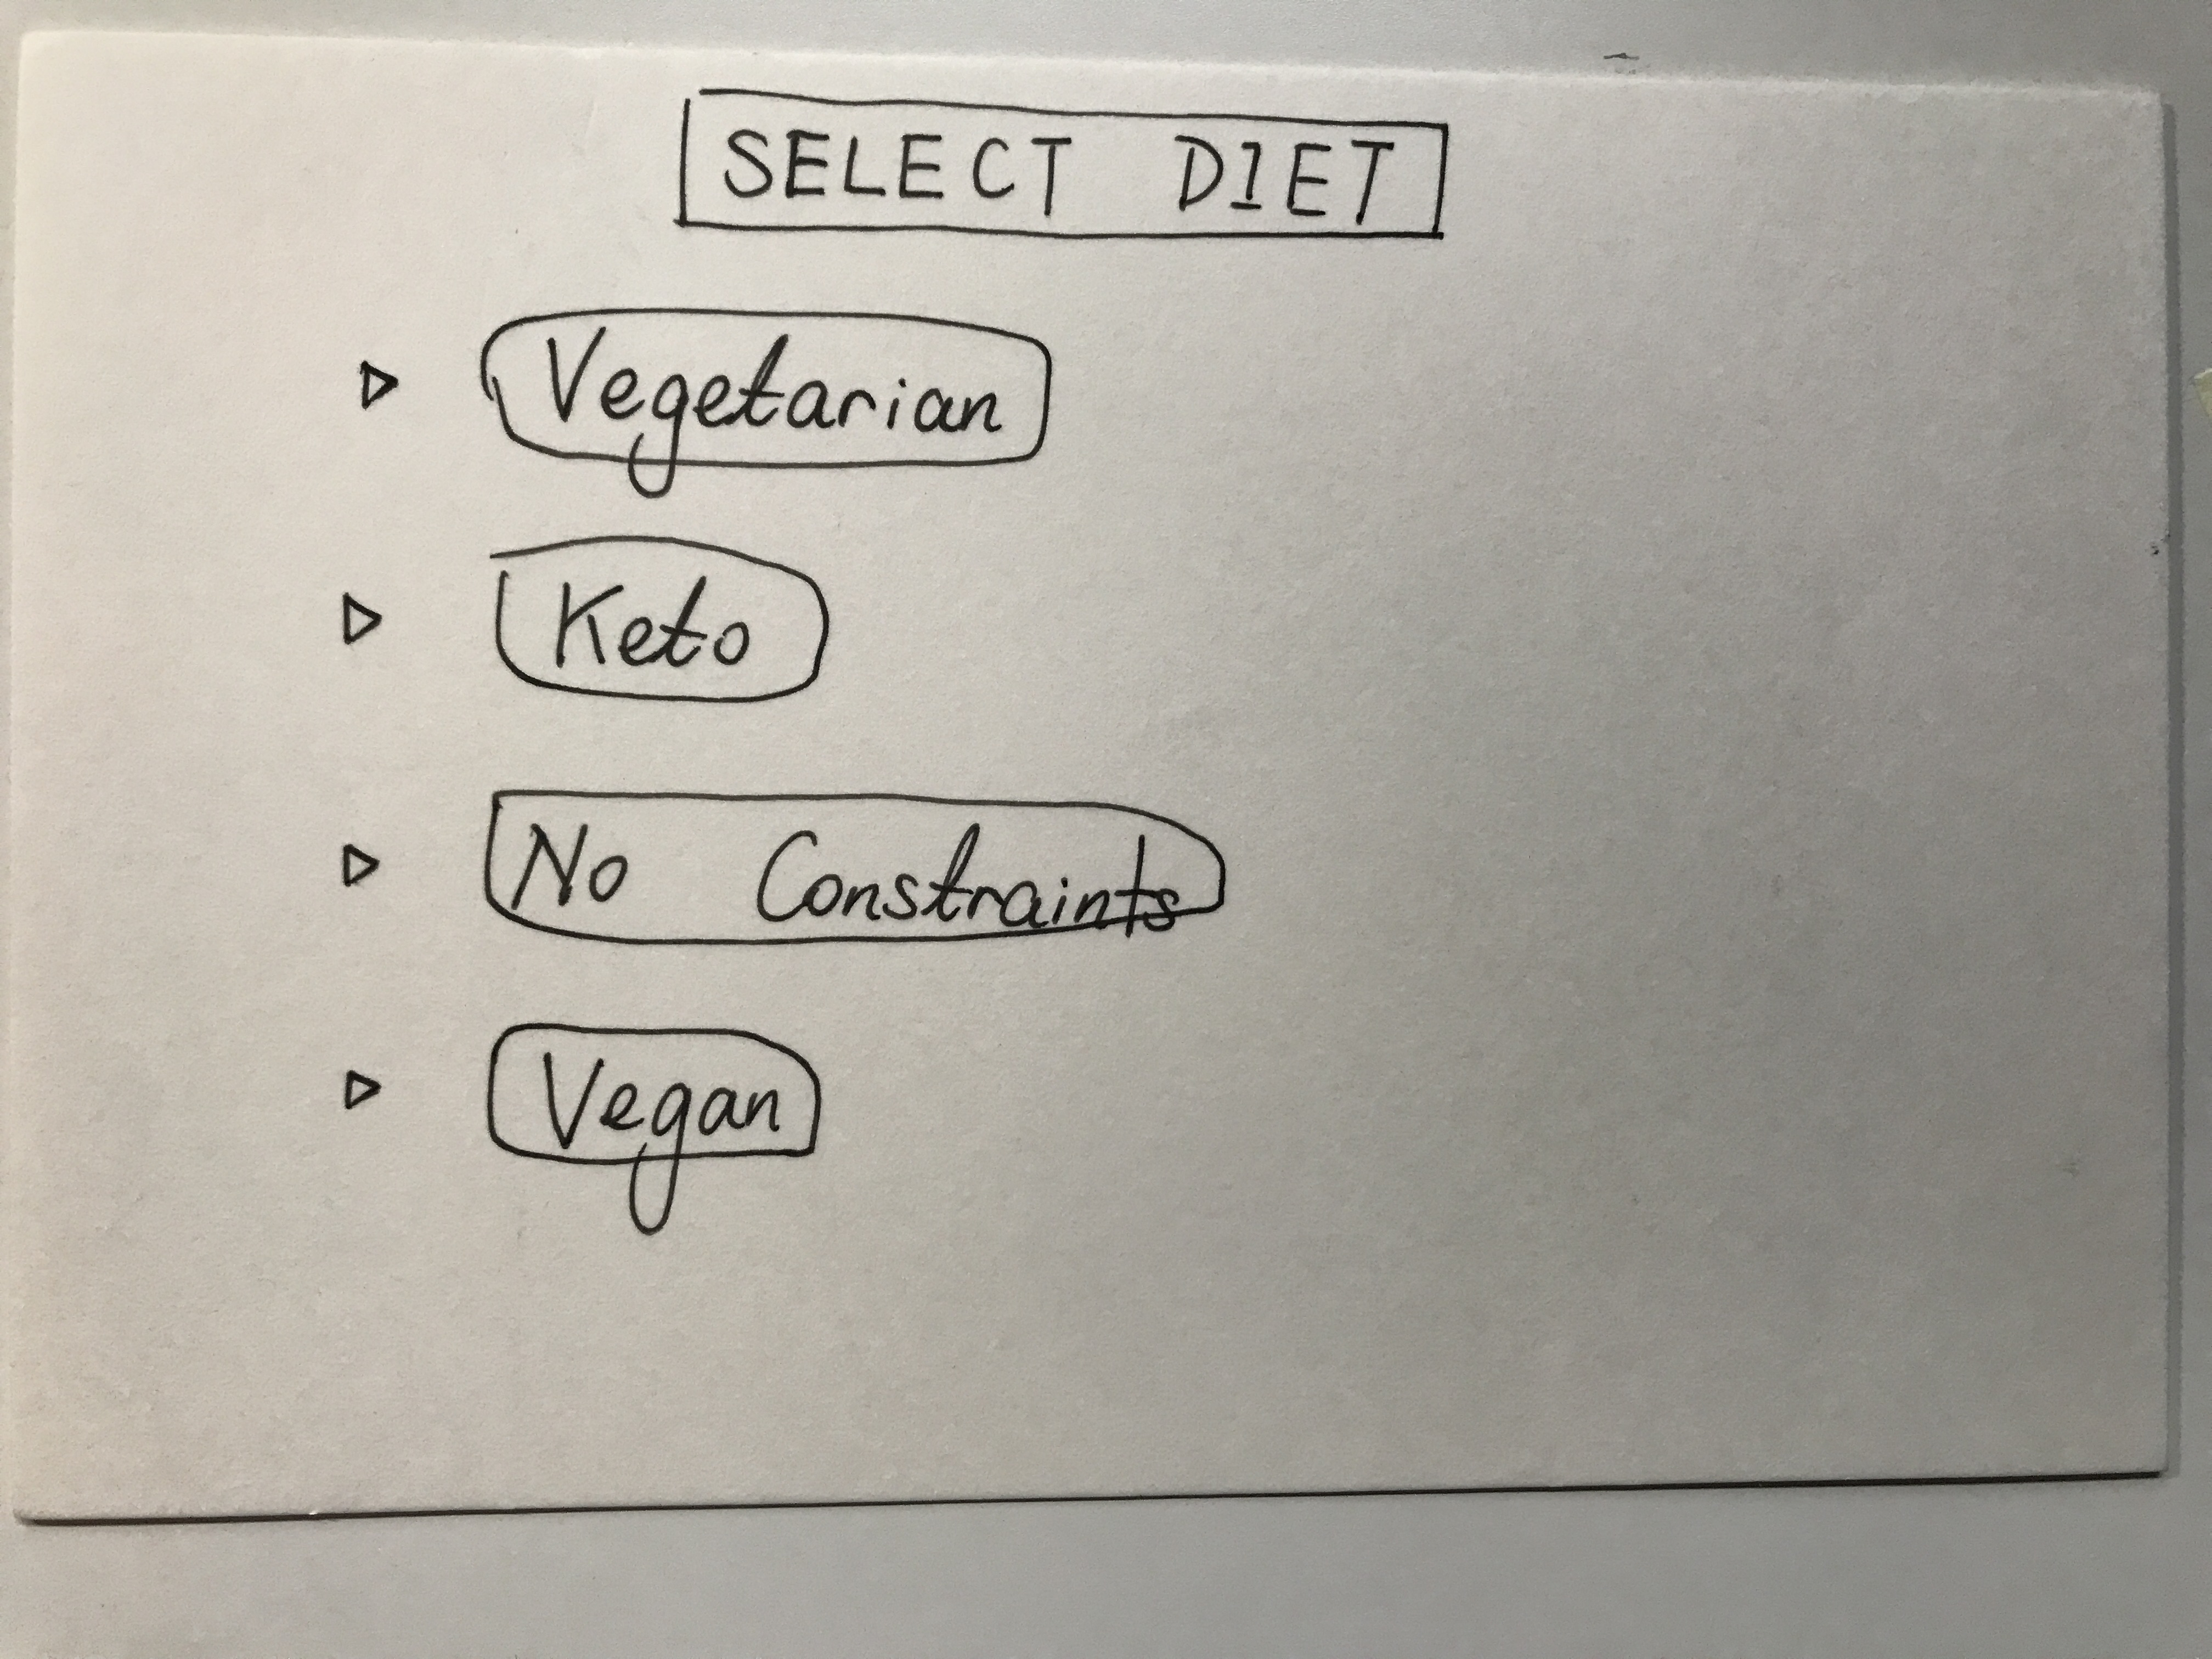
\includegraphics[scale=0.10, clip, trim={0em 0em 0em 0em}]{images/IMG_0561.jpg}
\end{figure}

\begin{figure}[h]
	\centering
	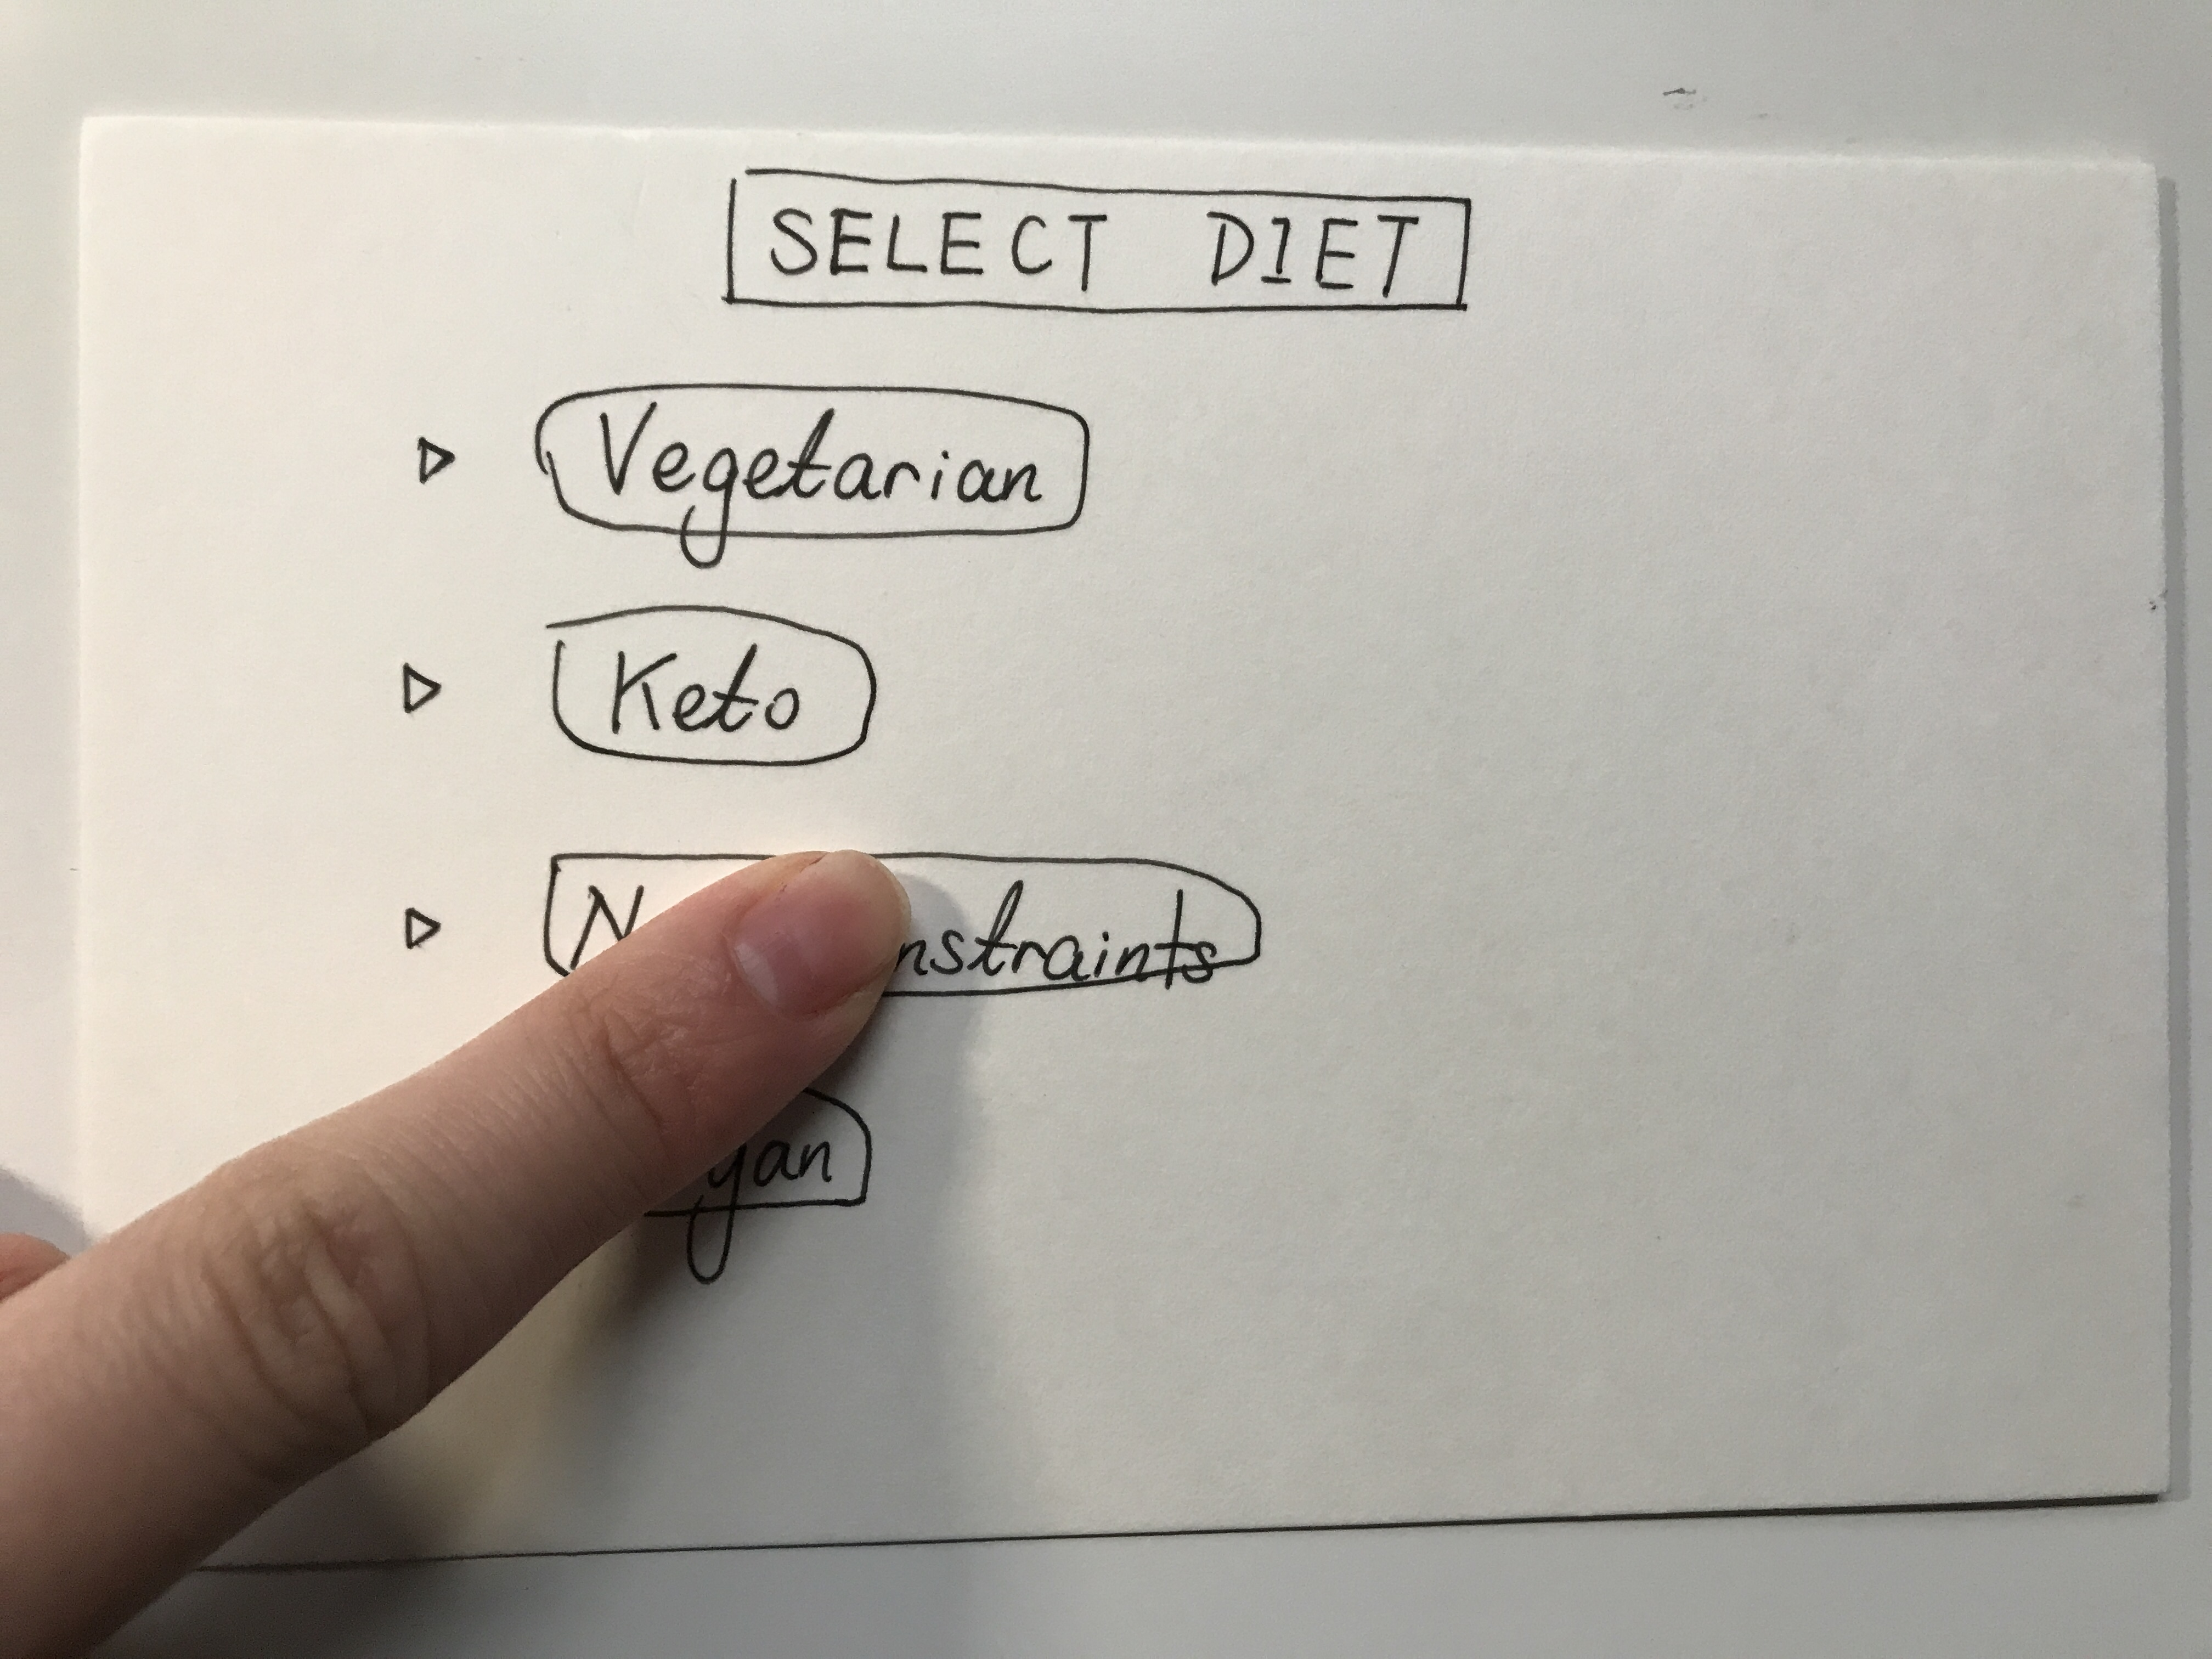
\includegraphics[scale=0.10, clip, trim={0em 0em 0em 0em}]{images/IMG_0563.jpg}
\end{figure}

\begin{figure}[h]
	\centering
	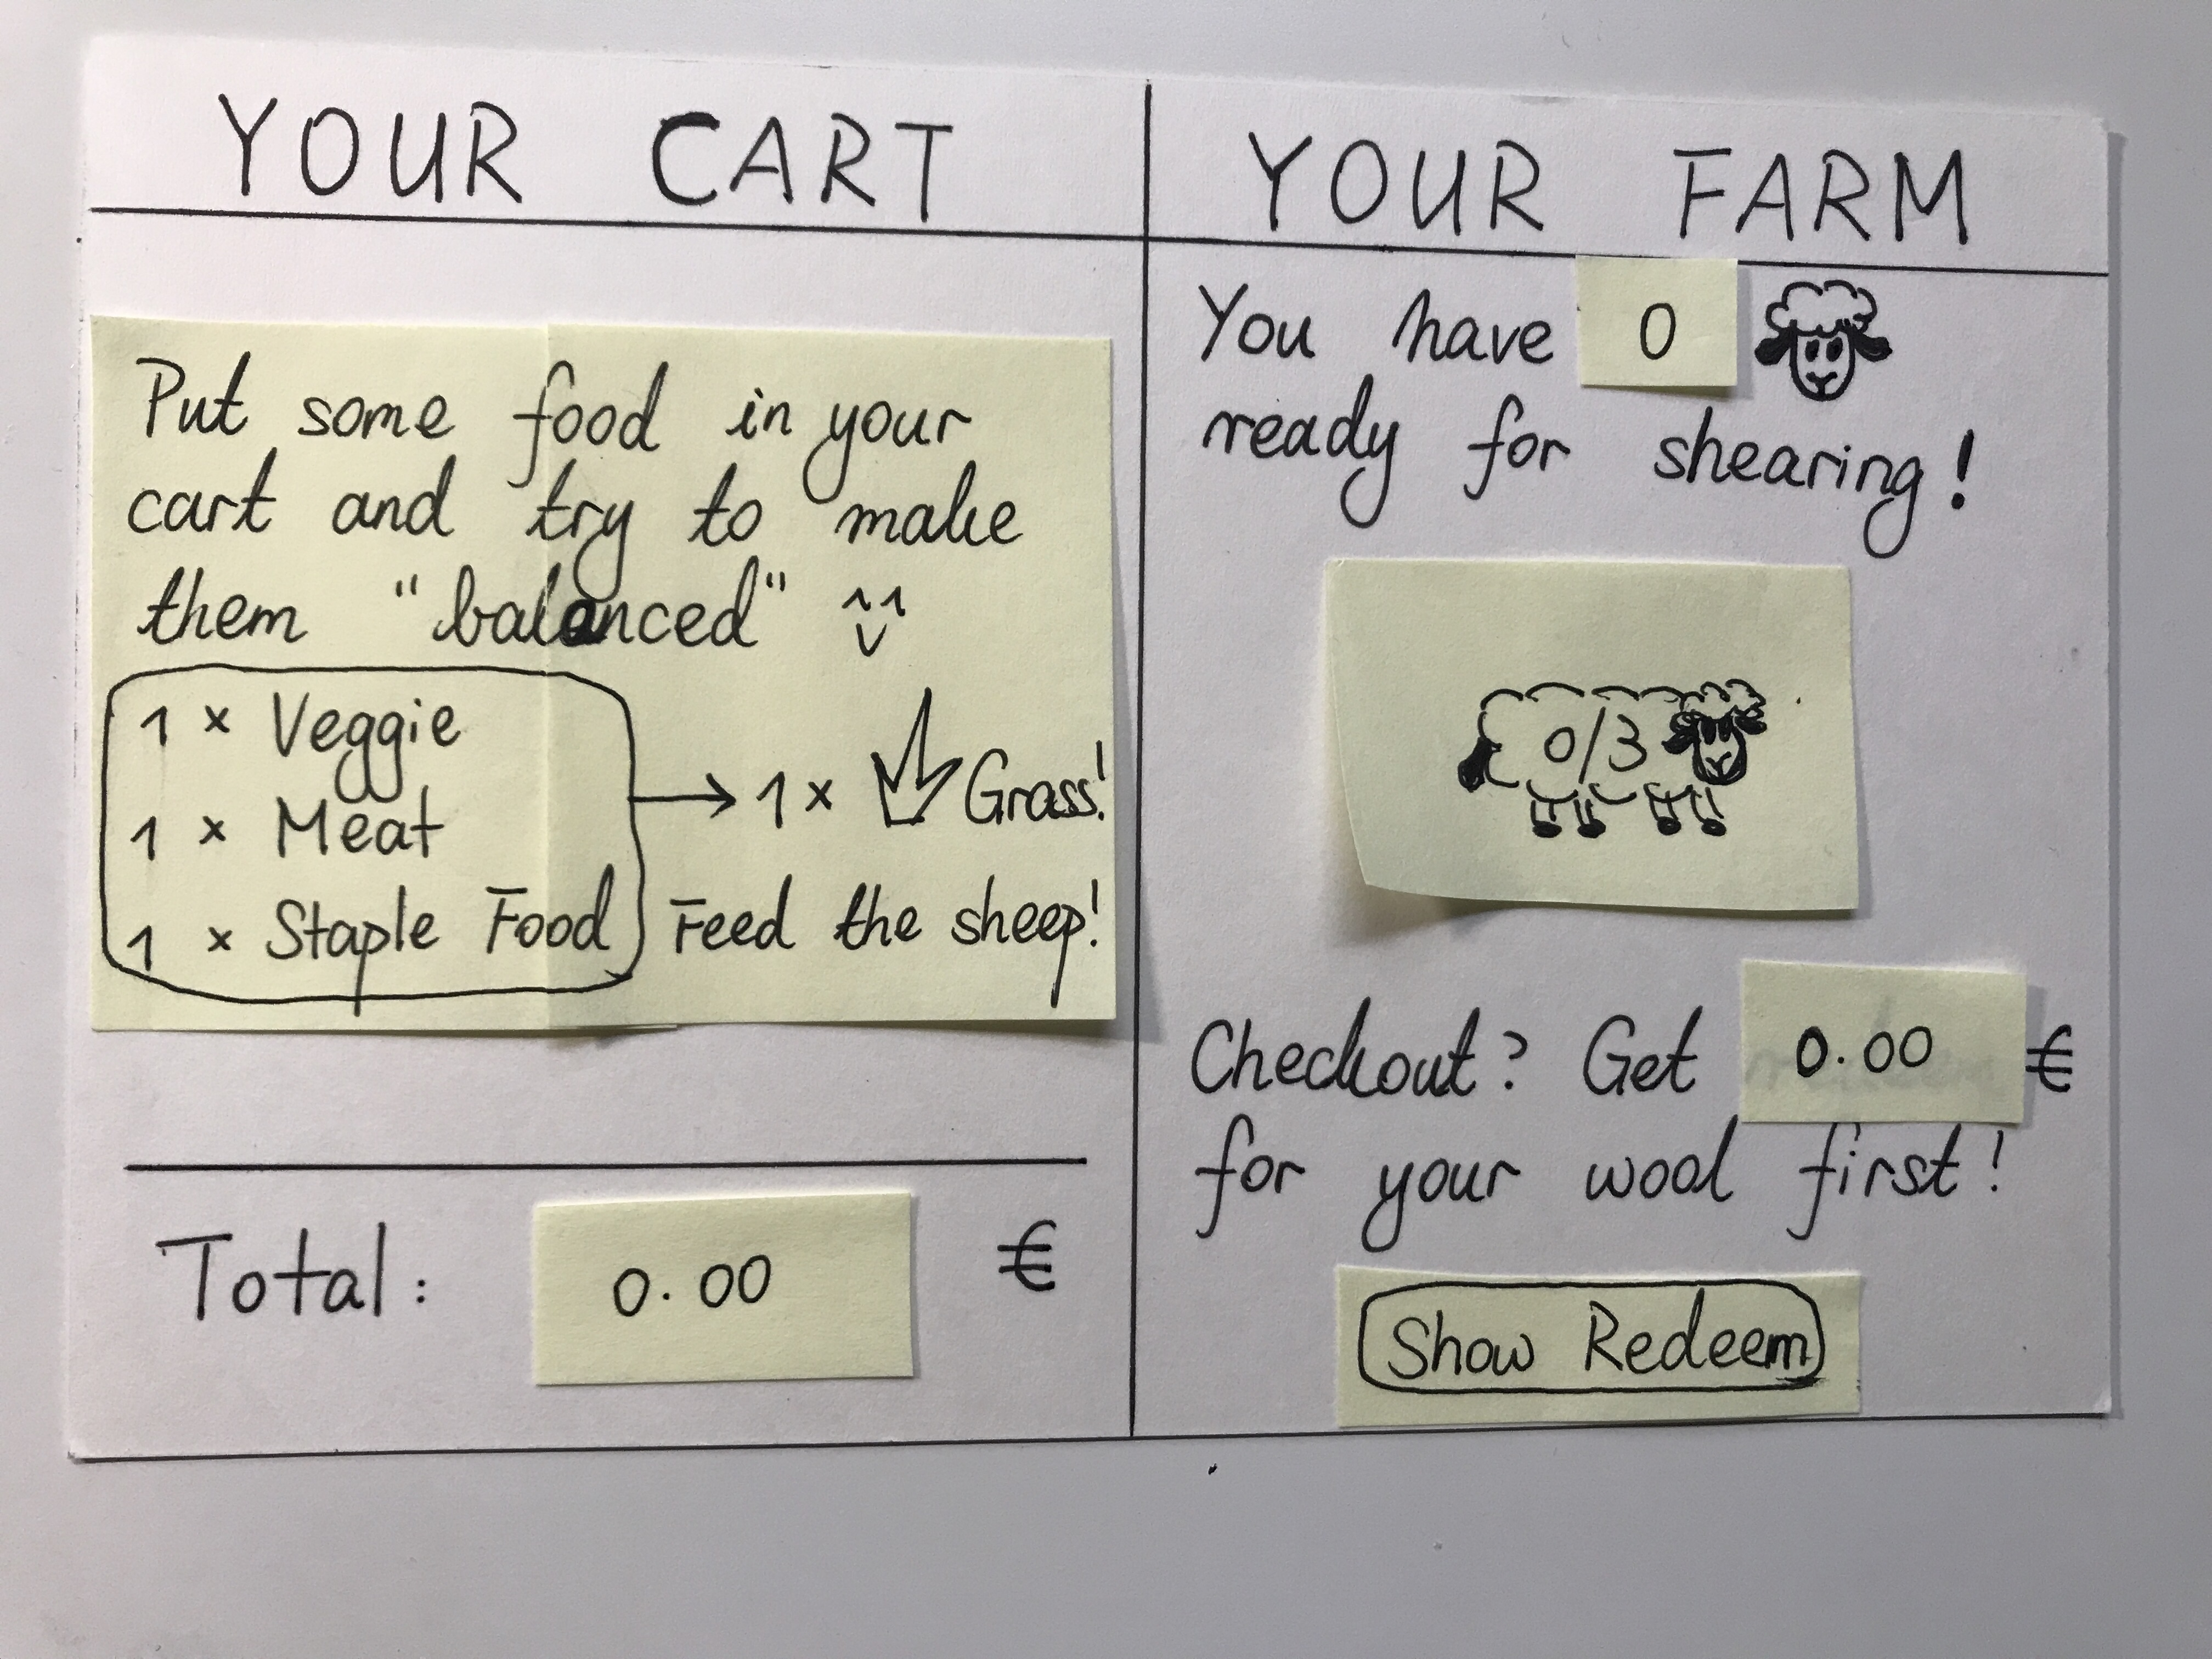
\includegraphics[scale=0.10, clip, trim={0em 0em 0em 0em}]{images/IMG_0565.jpg}
\end{figure}

\begin{figure}[h]
	\centering
	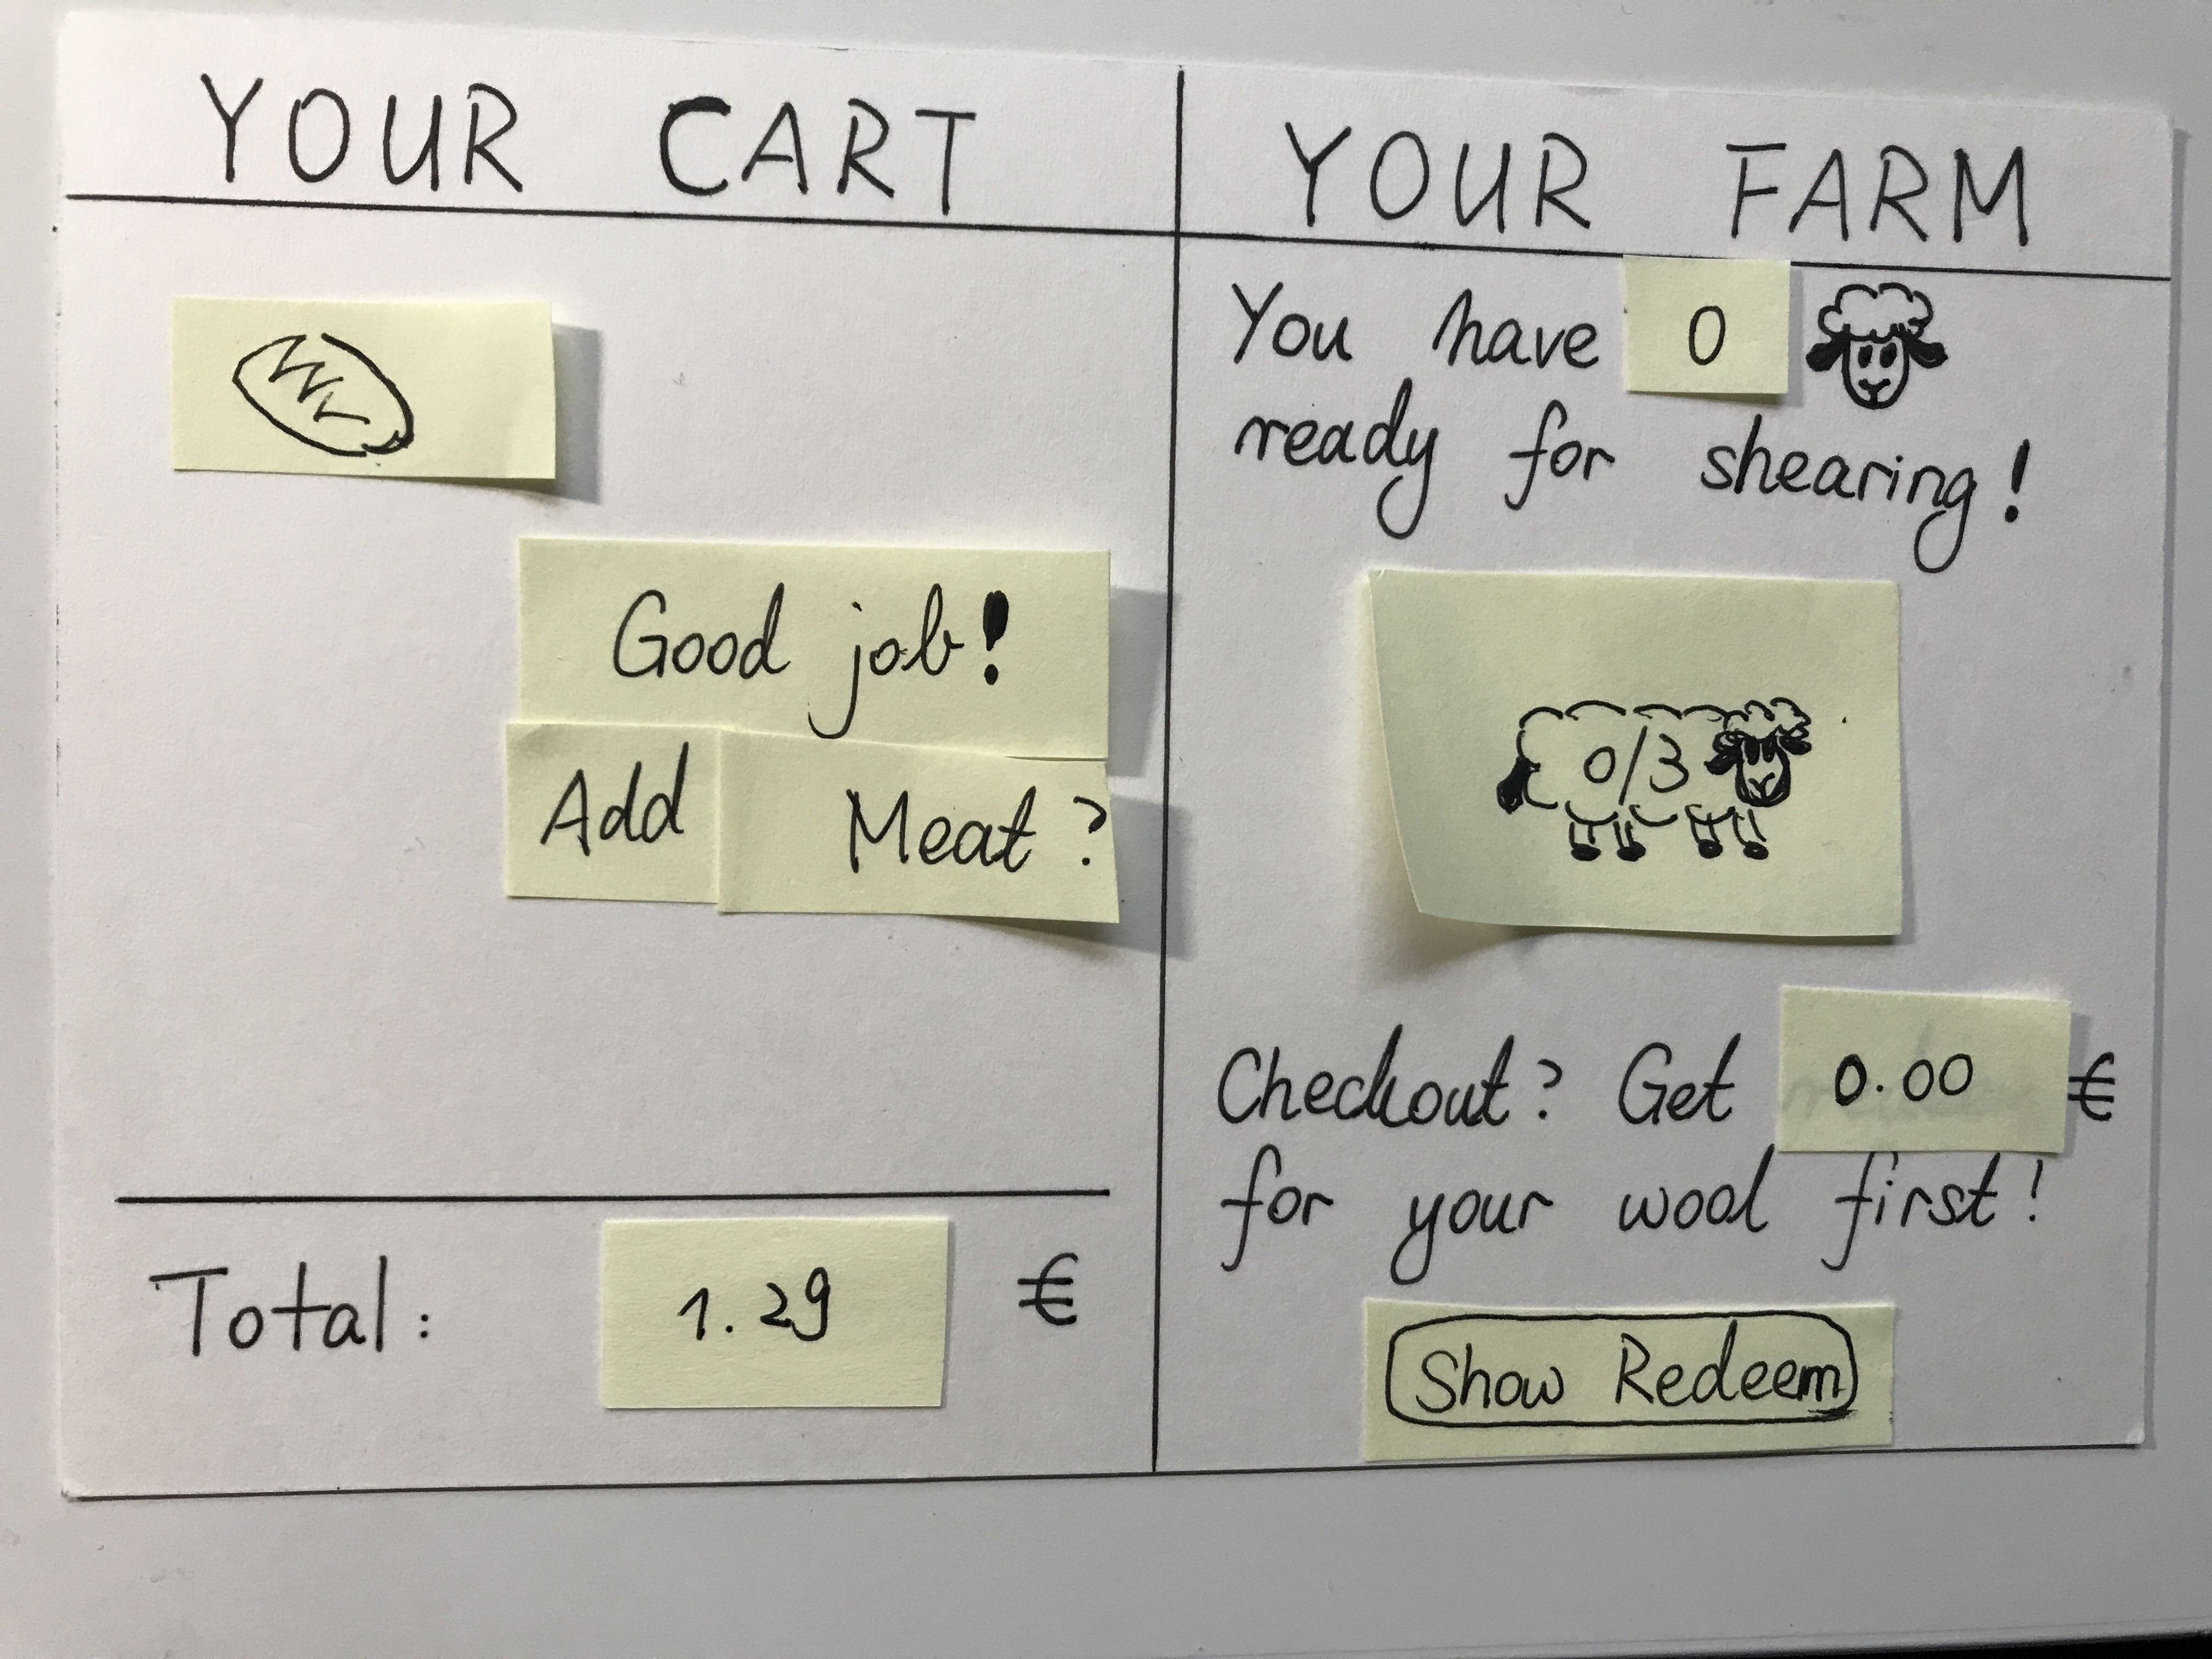
\includegraphics[scale=0.10, clip, trim={0em 0em 0em 0em}]{images/IMG_0566.jpg}
\end{figure}

\begin{figure}[h]
	\centering
	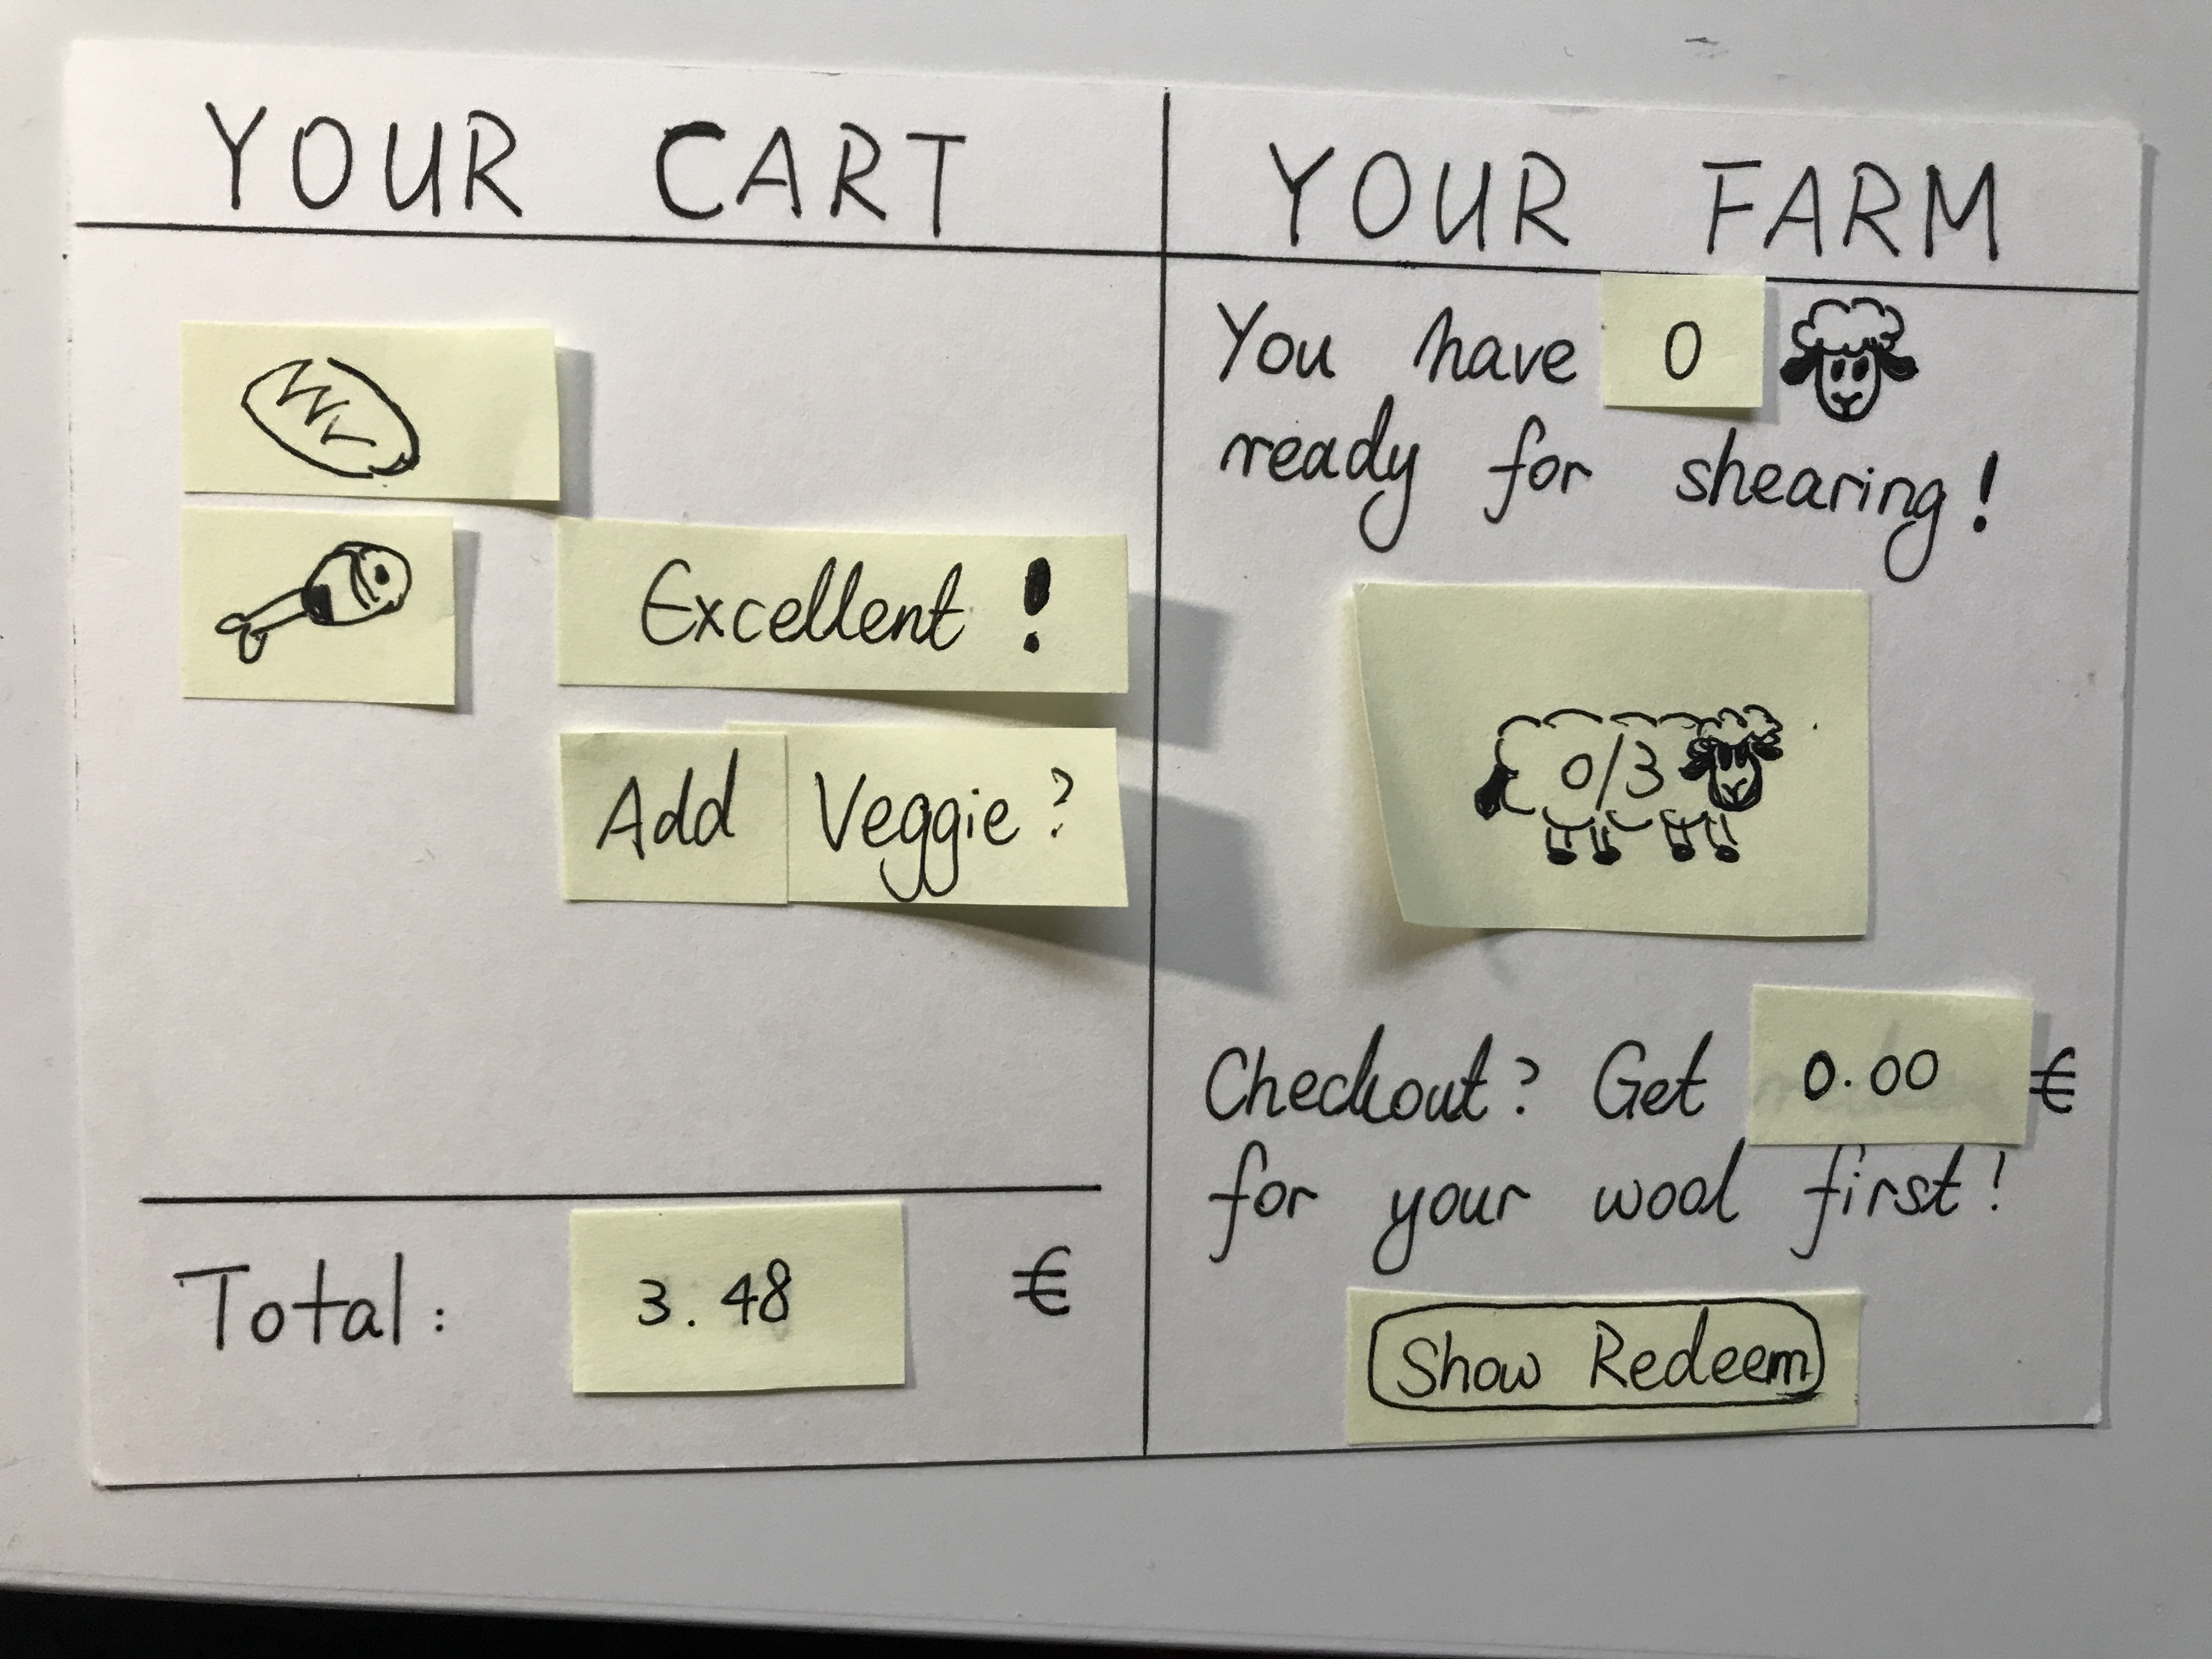
\includegraphics[scale=0.10, clip, trim={0em 0em 0em 0em}]{images/IMG_0567.jpg}
\end{figure}

\begin{figure}[h]
	\centering
	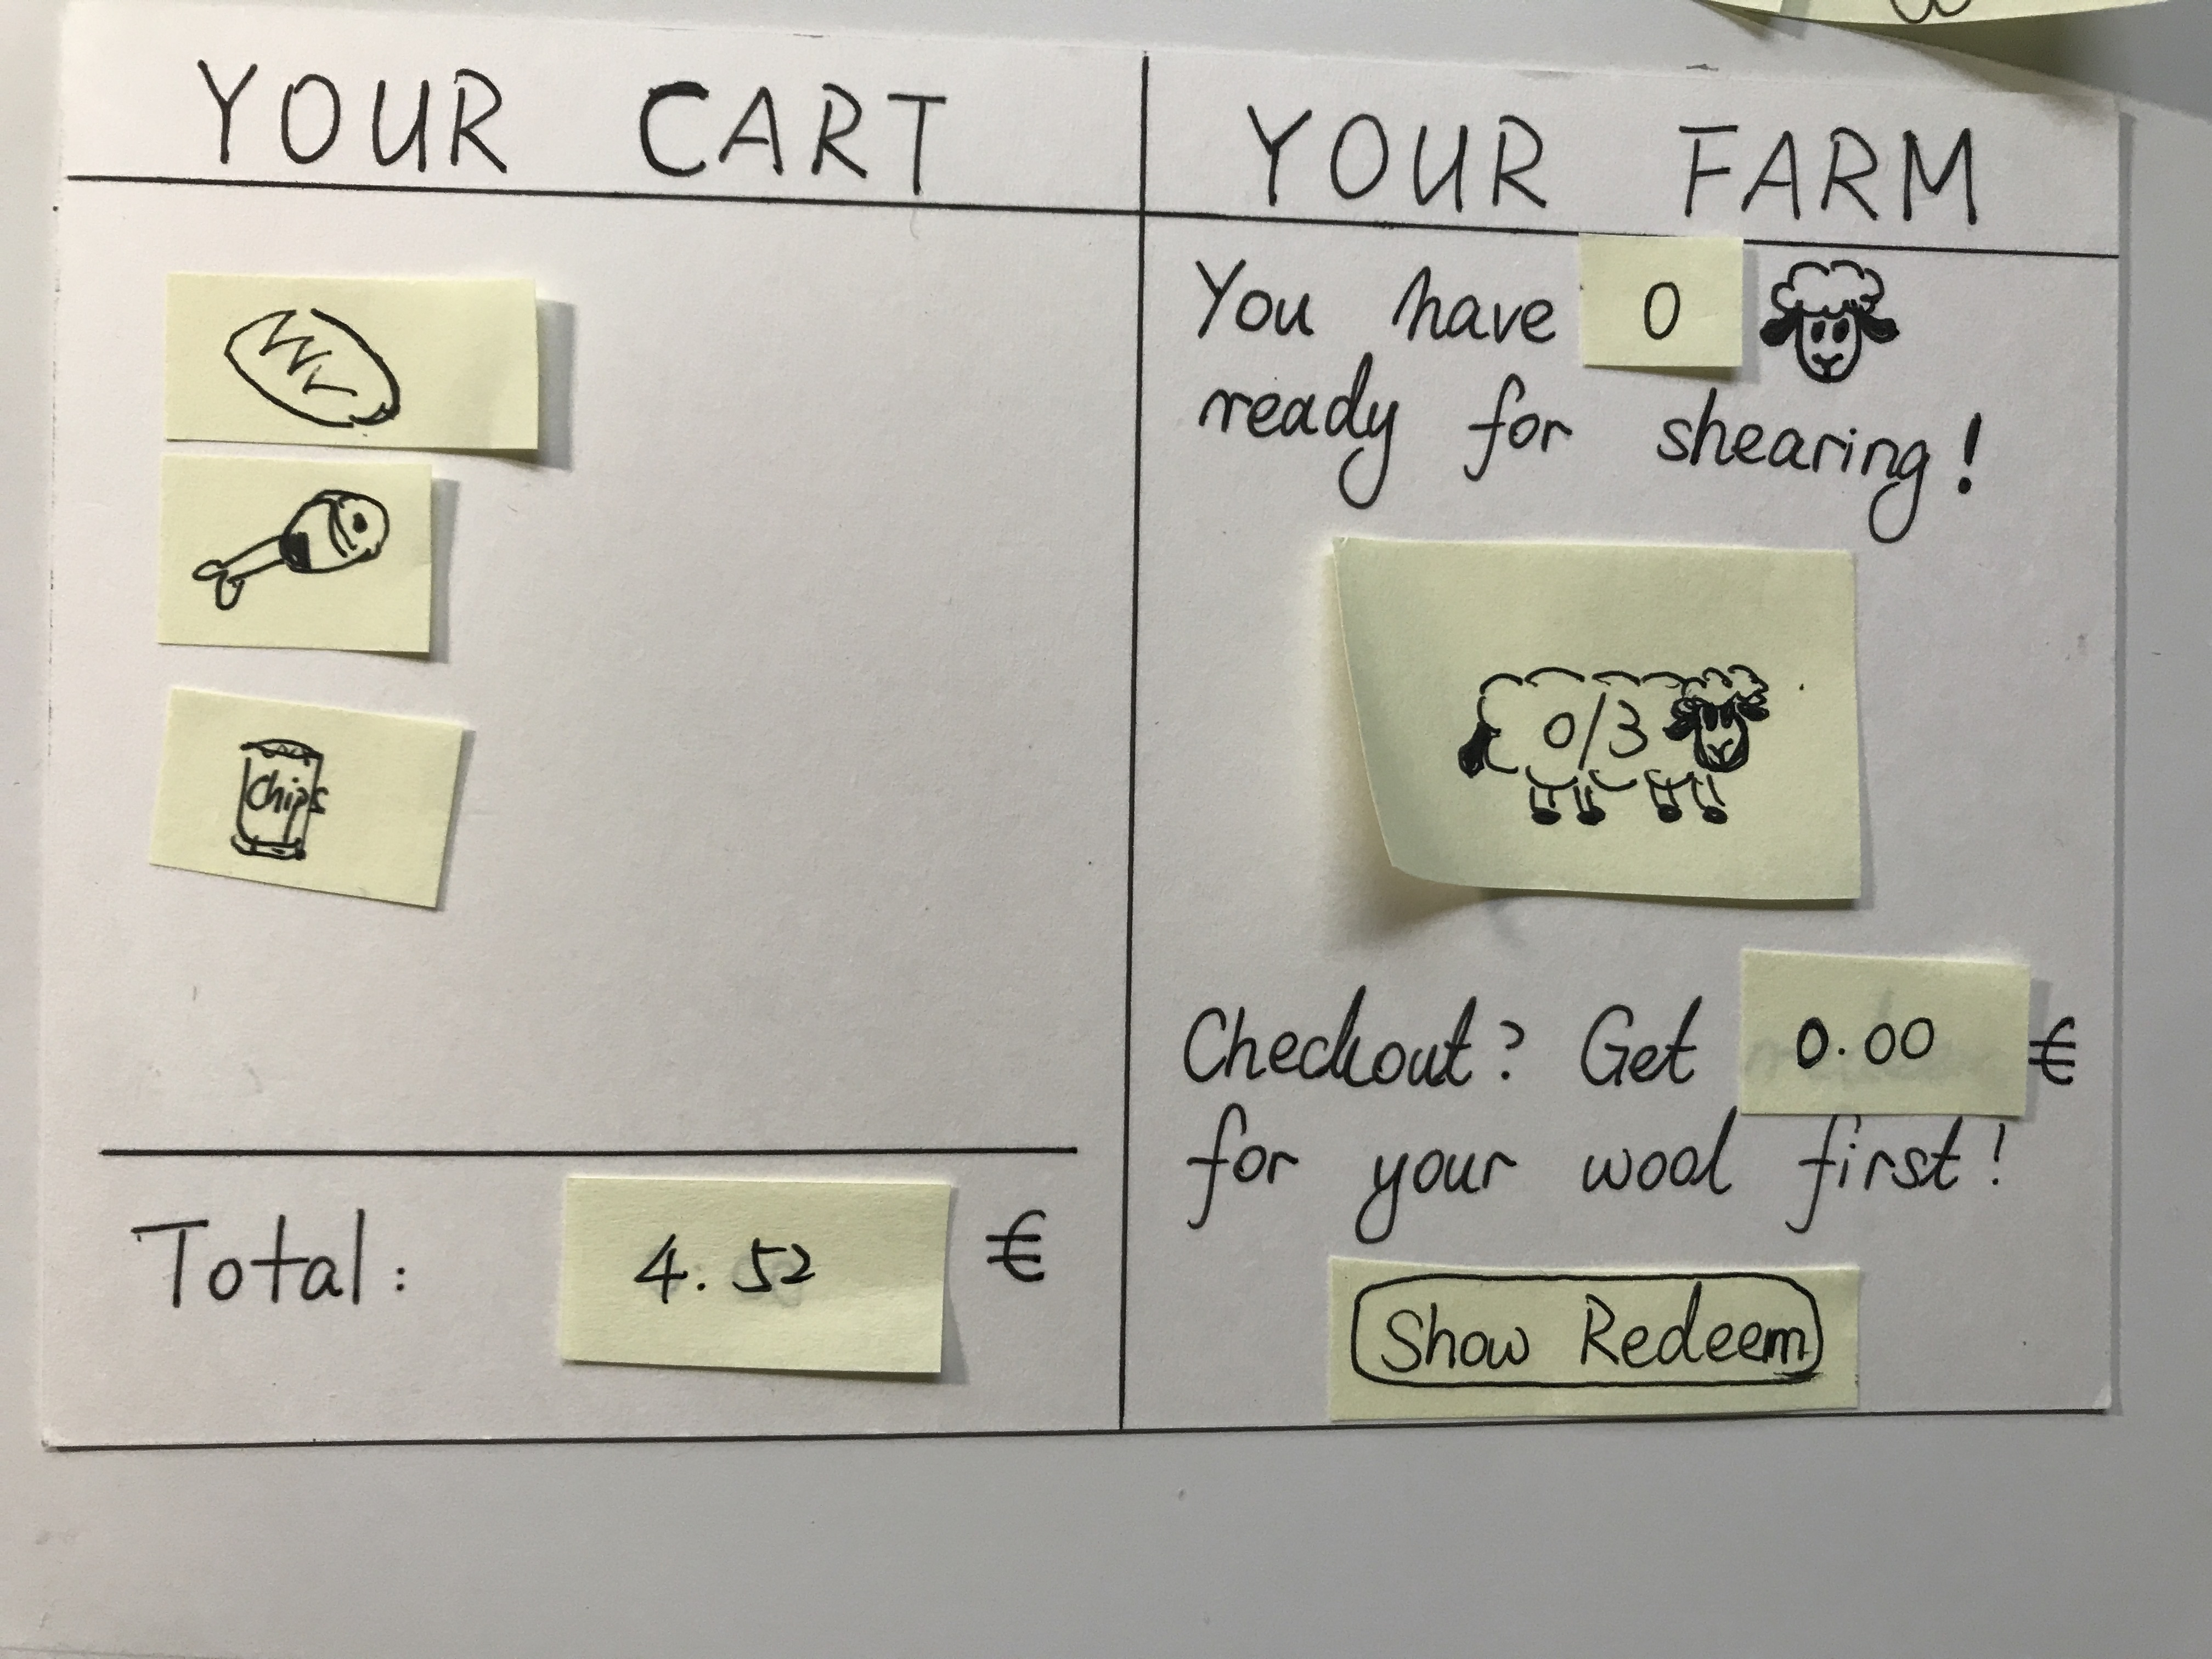
\includegraphics[scale=0.10, clip, trim={0em 0em 0em 0em}]{images/IMG_0569.jpg}
\end{figure}

\begin{figure}[h]
	\centering
	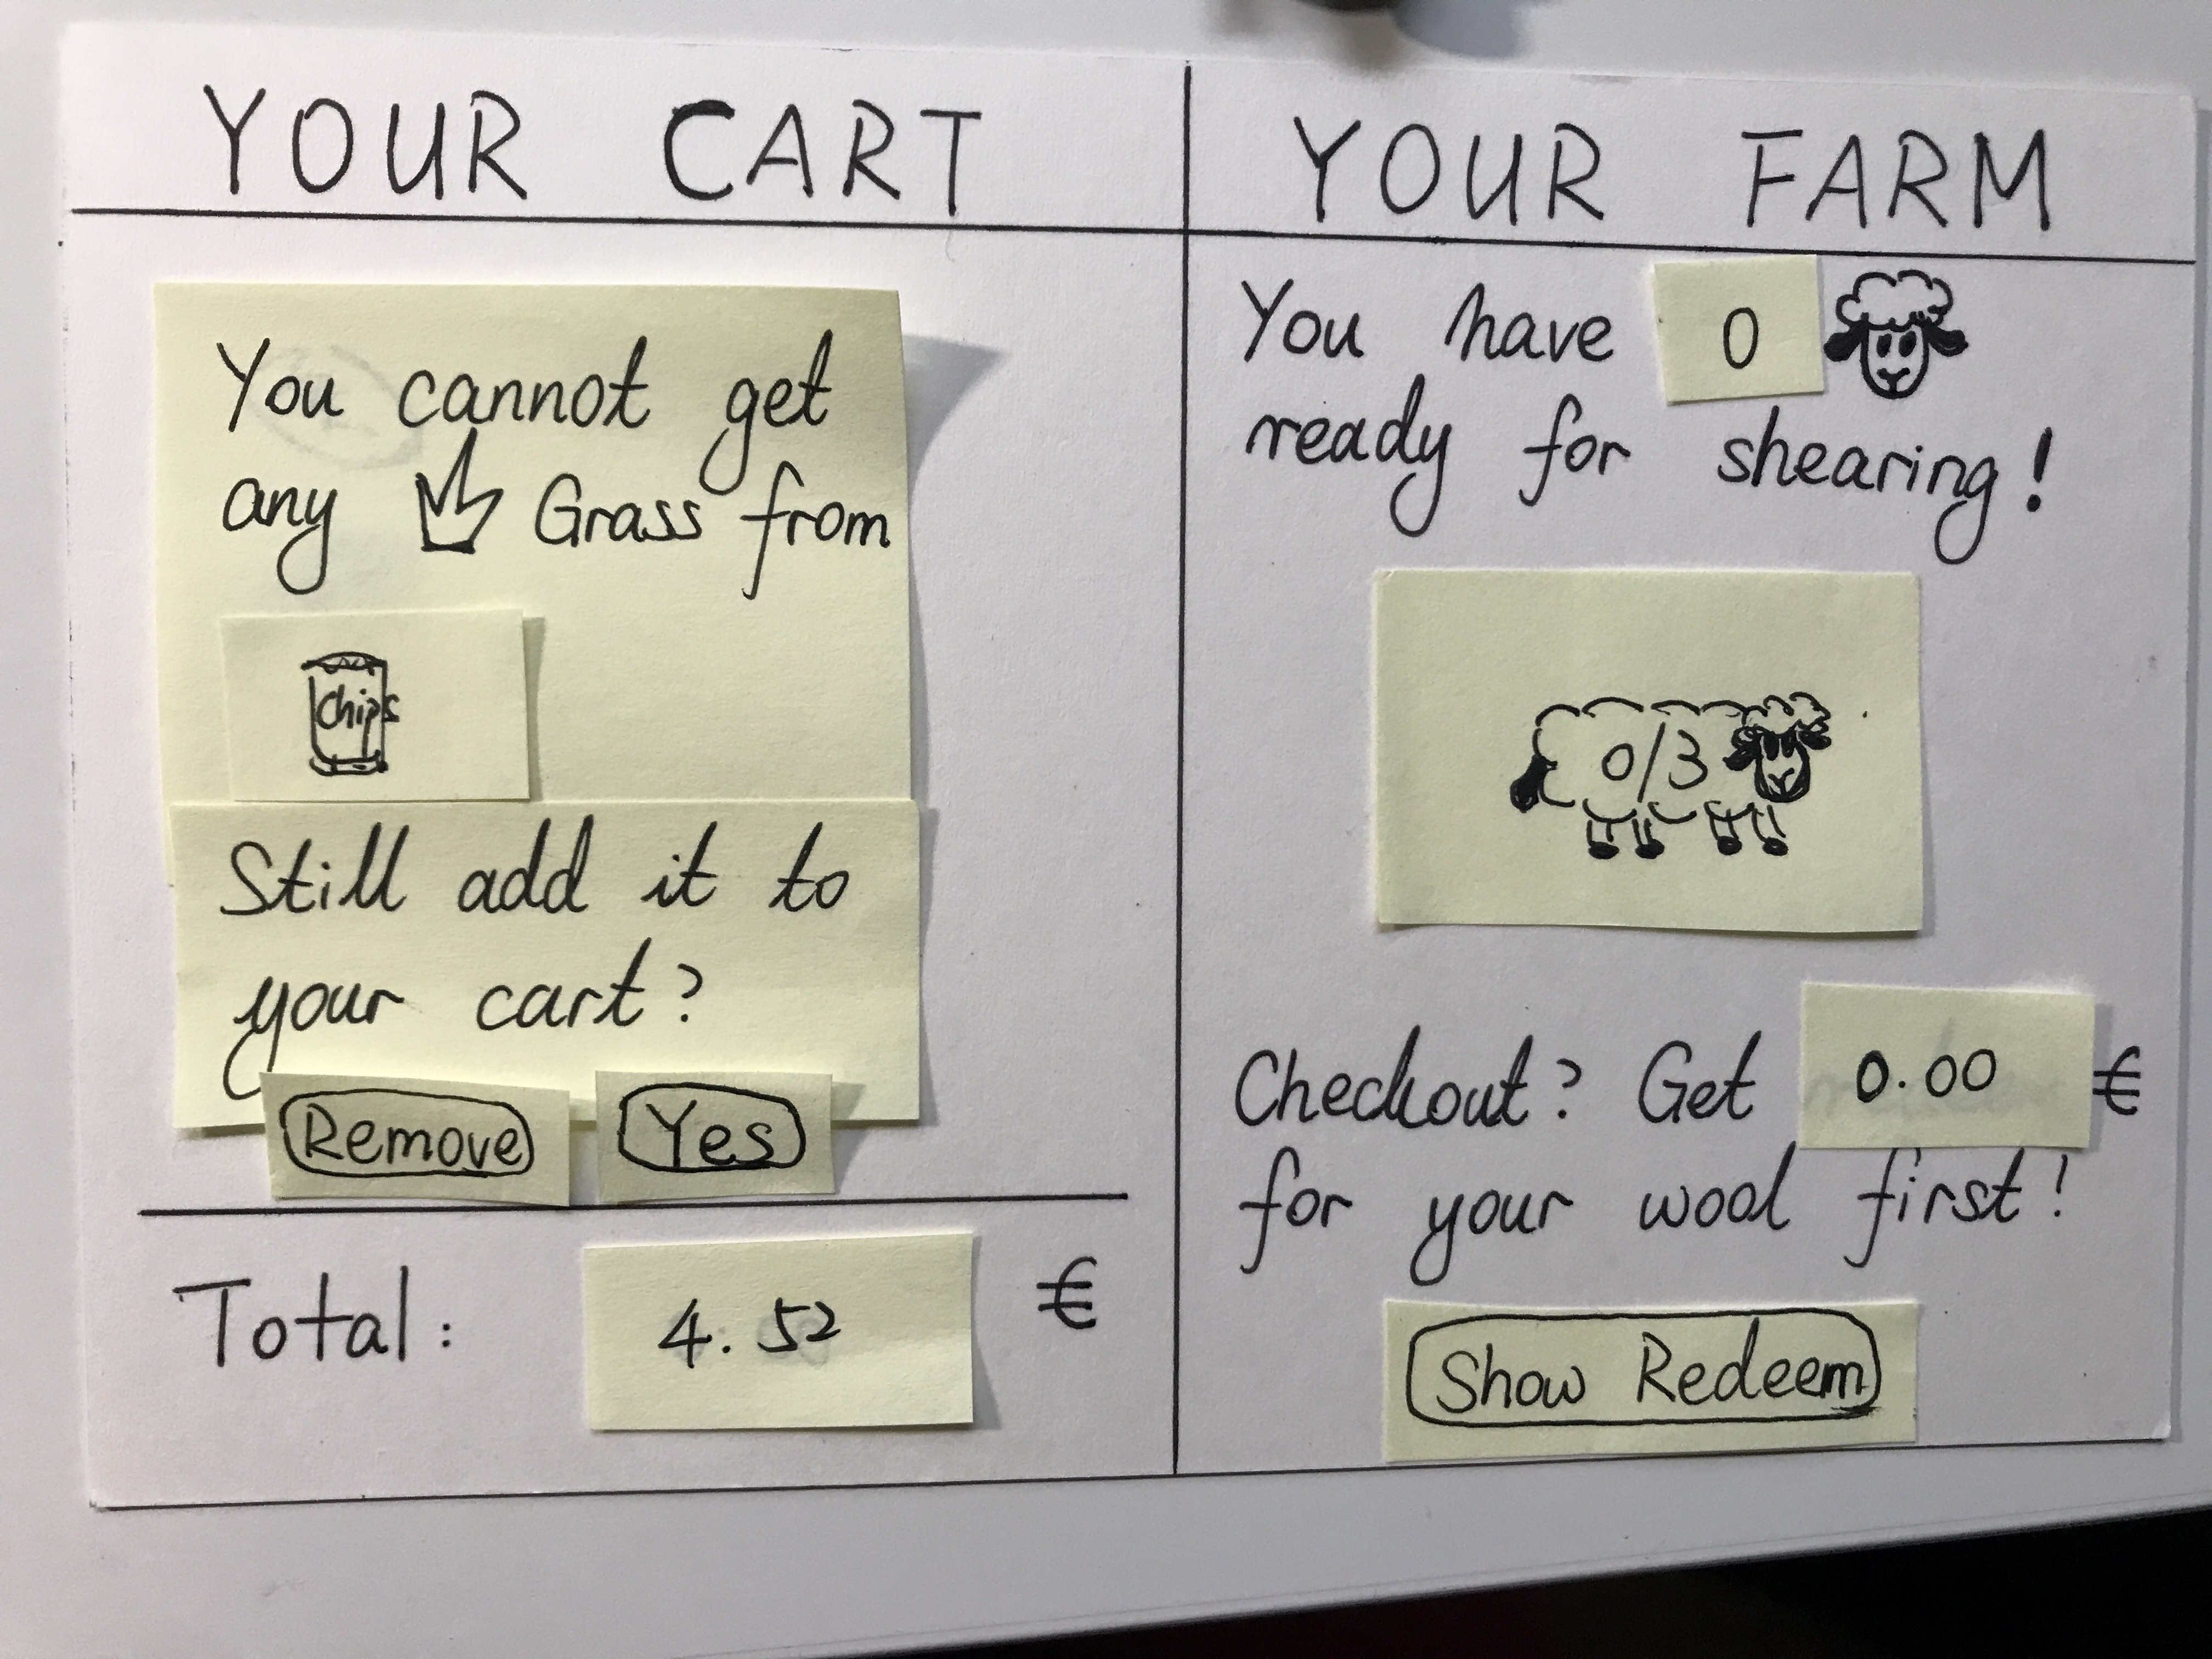
\includegraphics[scale=0.10, clip, trim={0em 0em 0em 0em}]{images/IMG_0570.jpg}
\end{figure}

\begin{figure}[h]
	\centering
	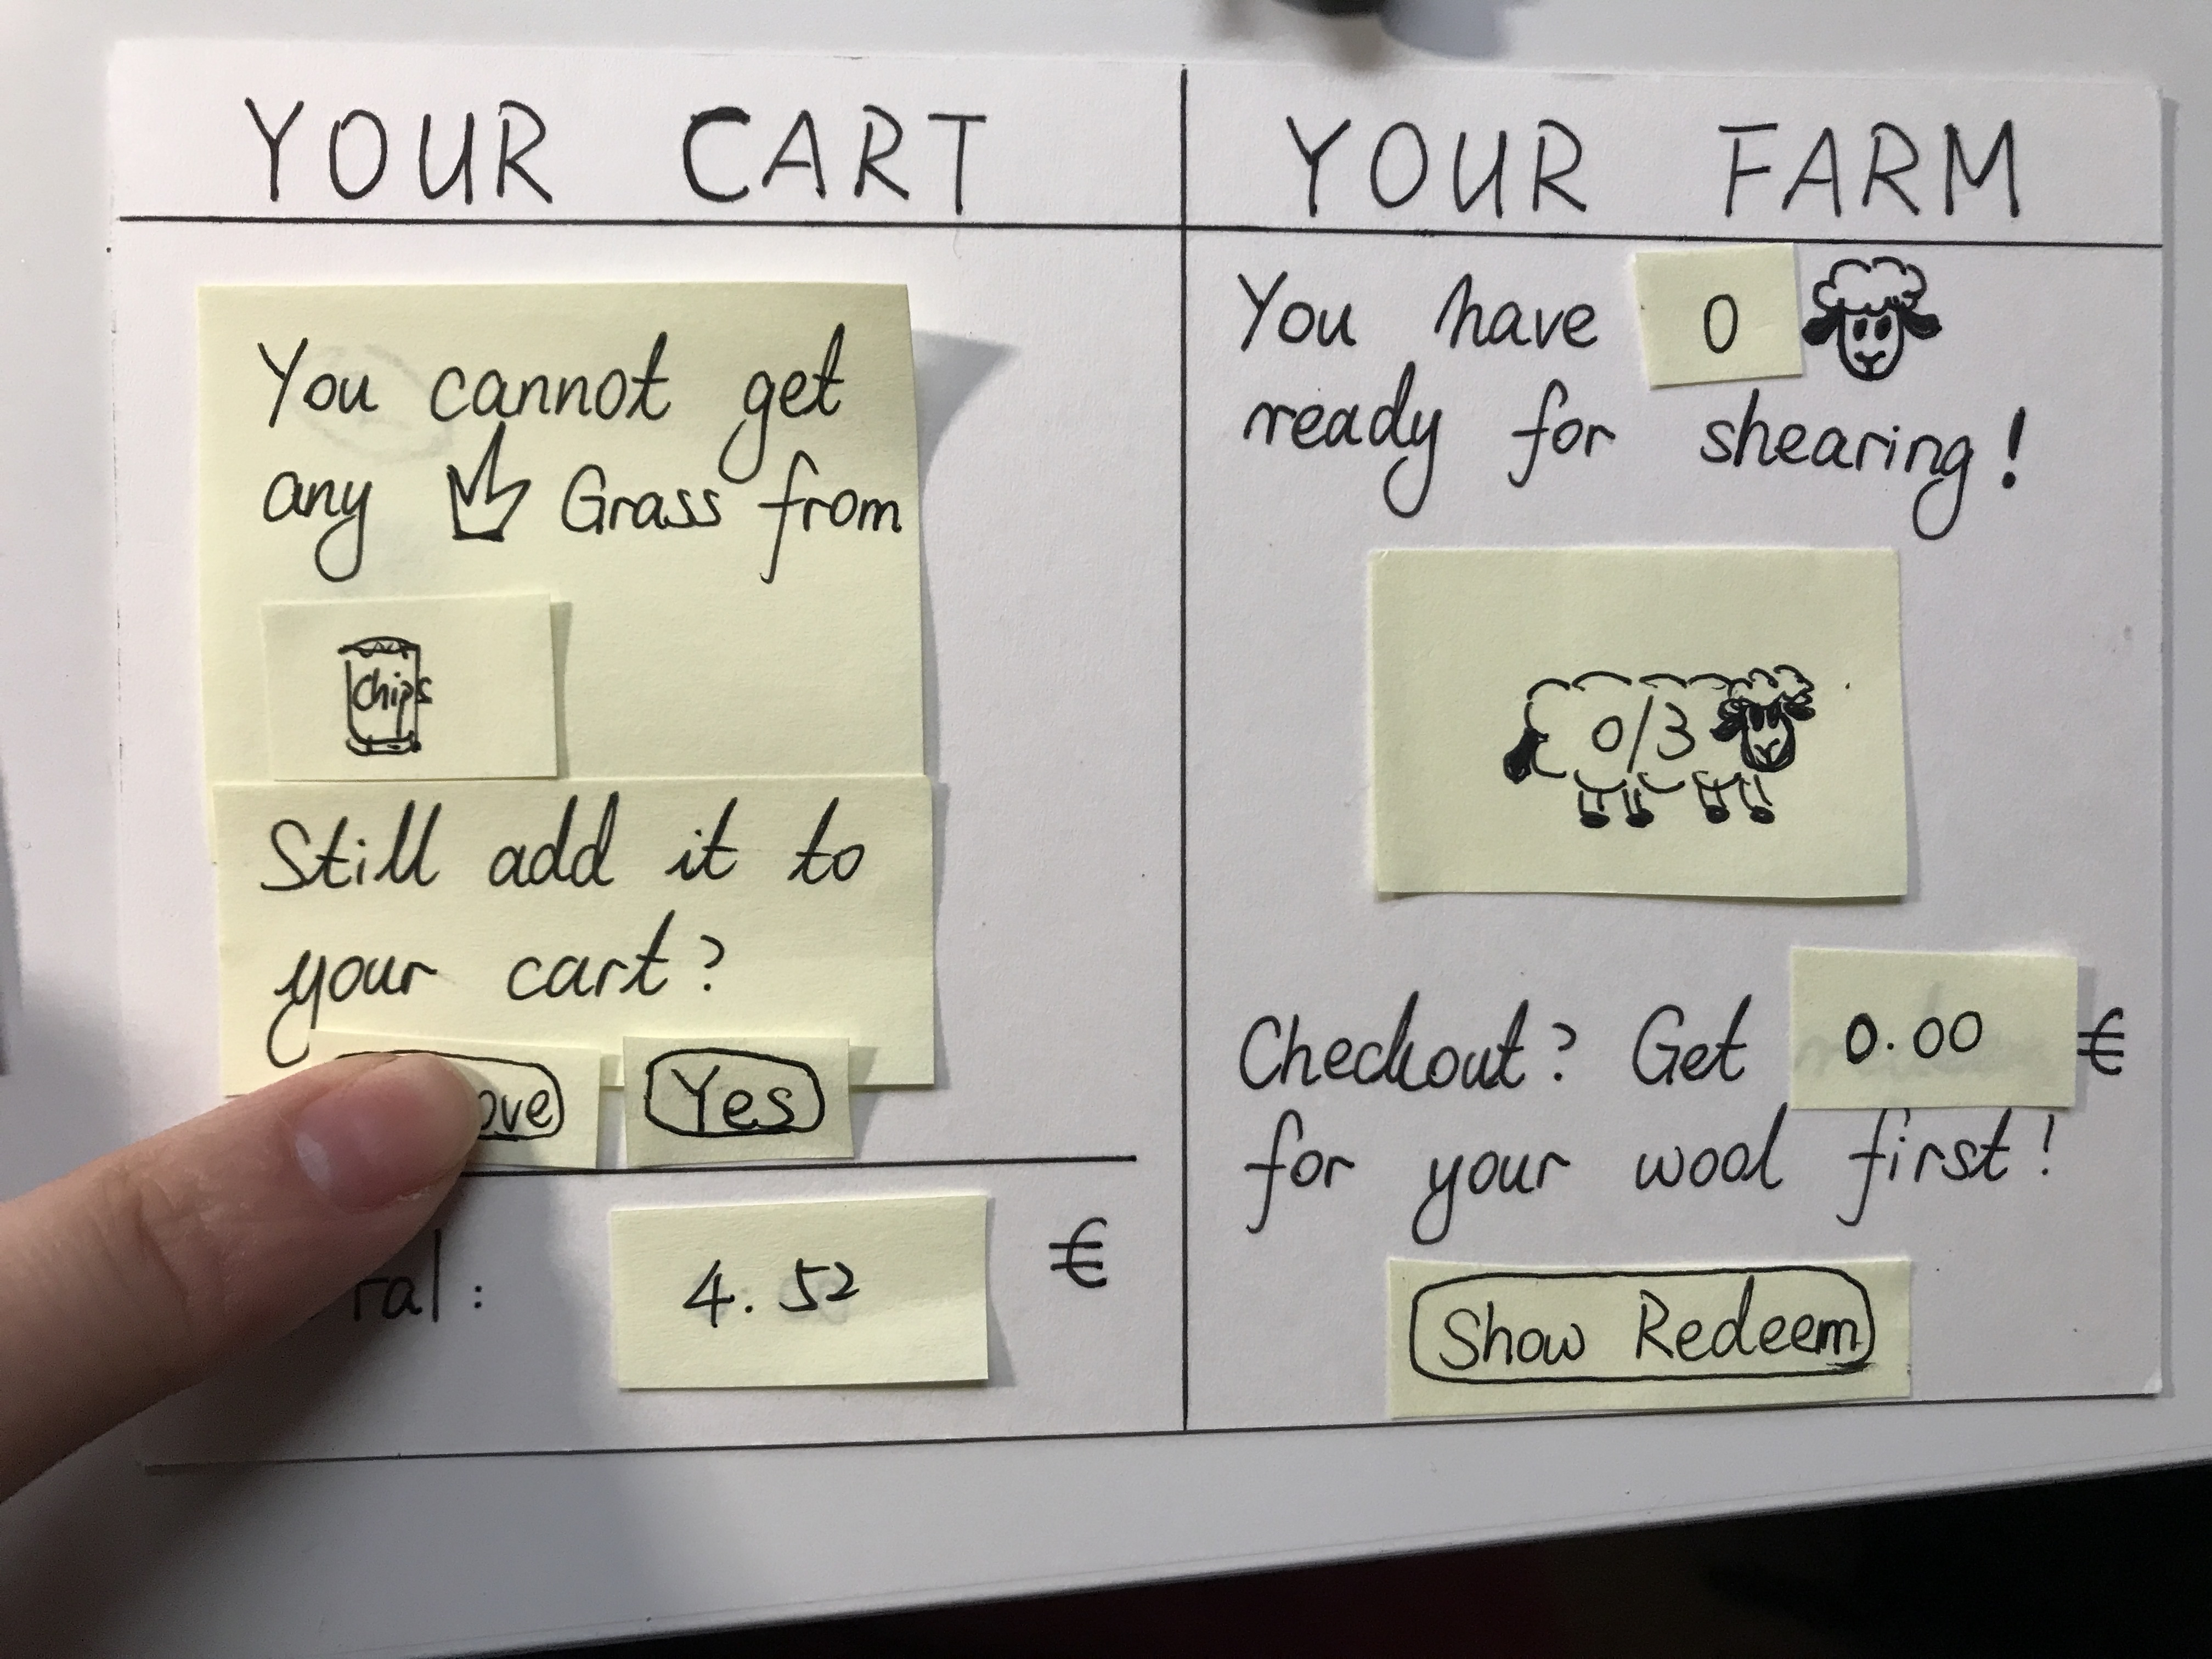
\includegraphics[scale=0.10, clip, trim={0em 0em 0em 0em}]{images/IMG_0571.jpg}
\end{figure}

\begin{figure}[h]
	\centering
	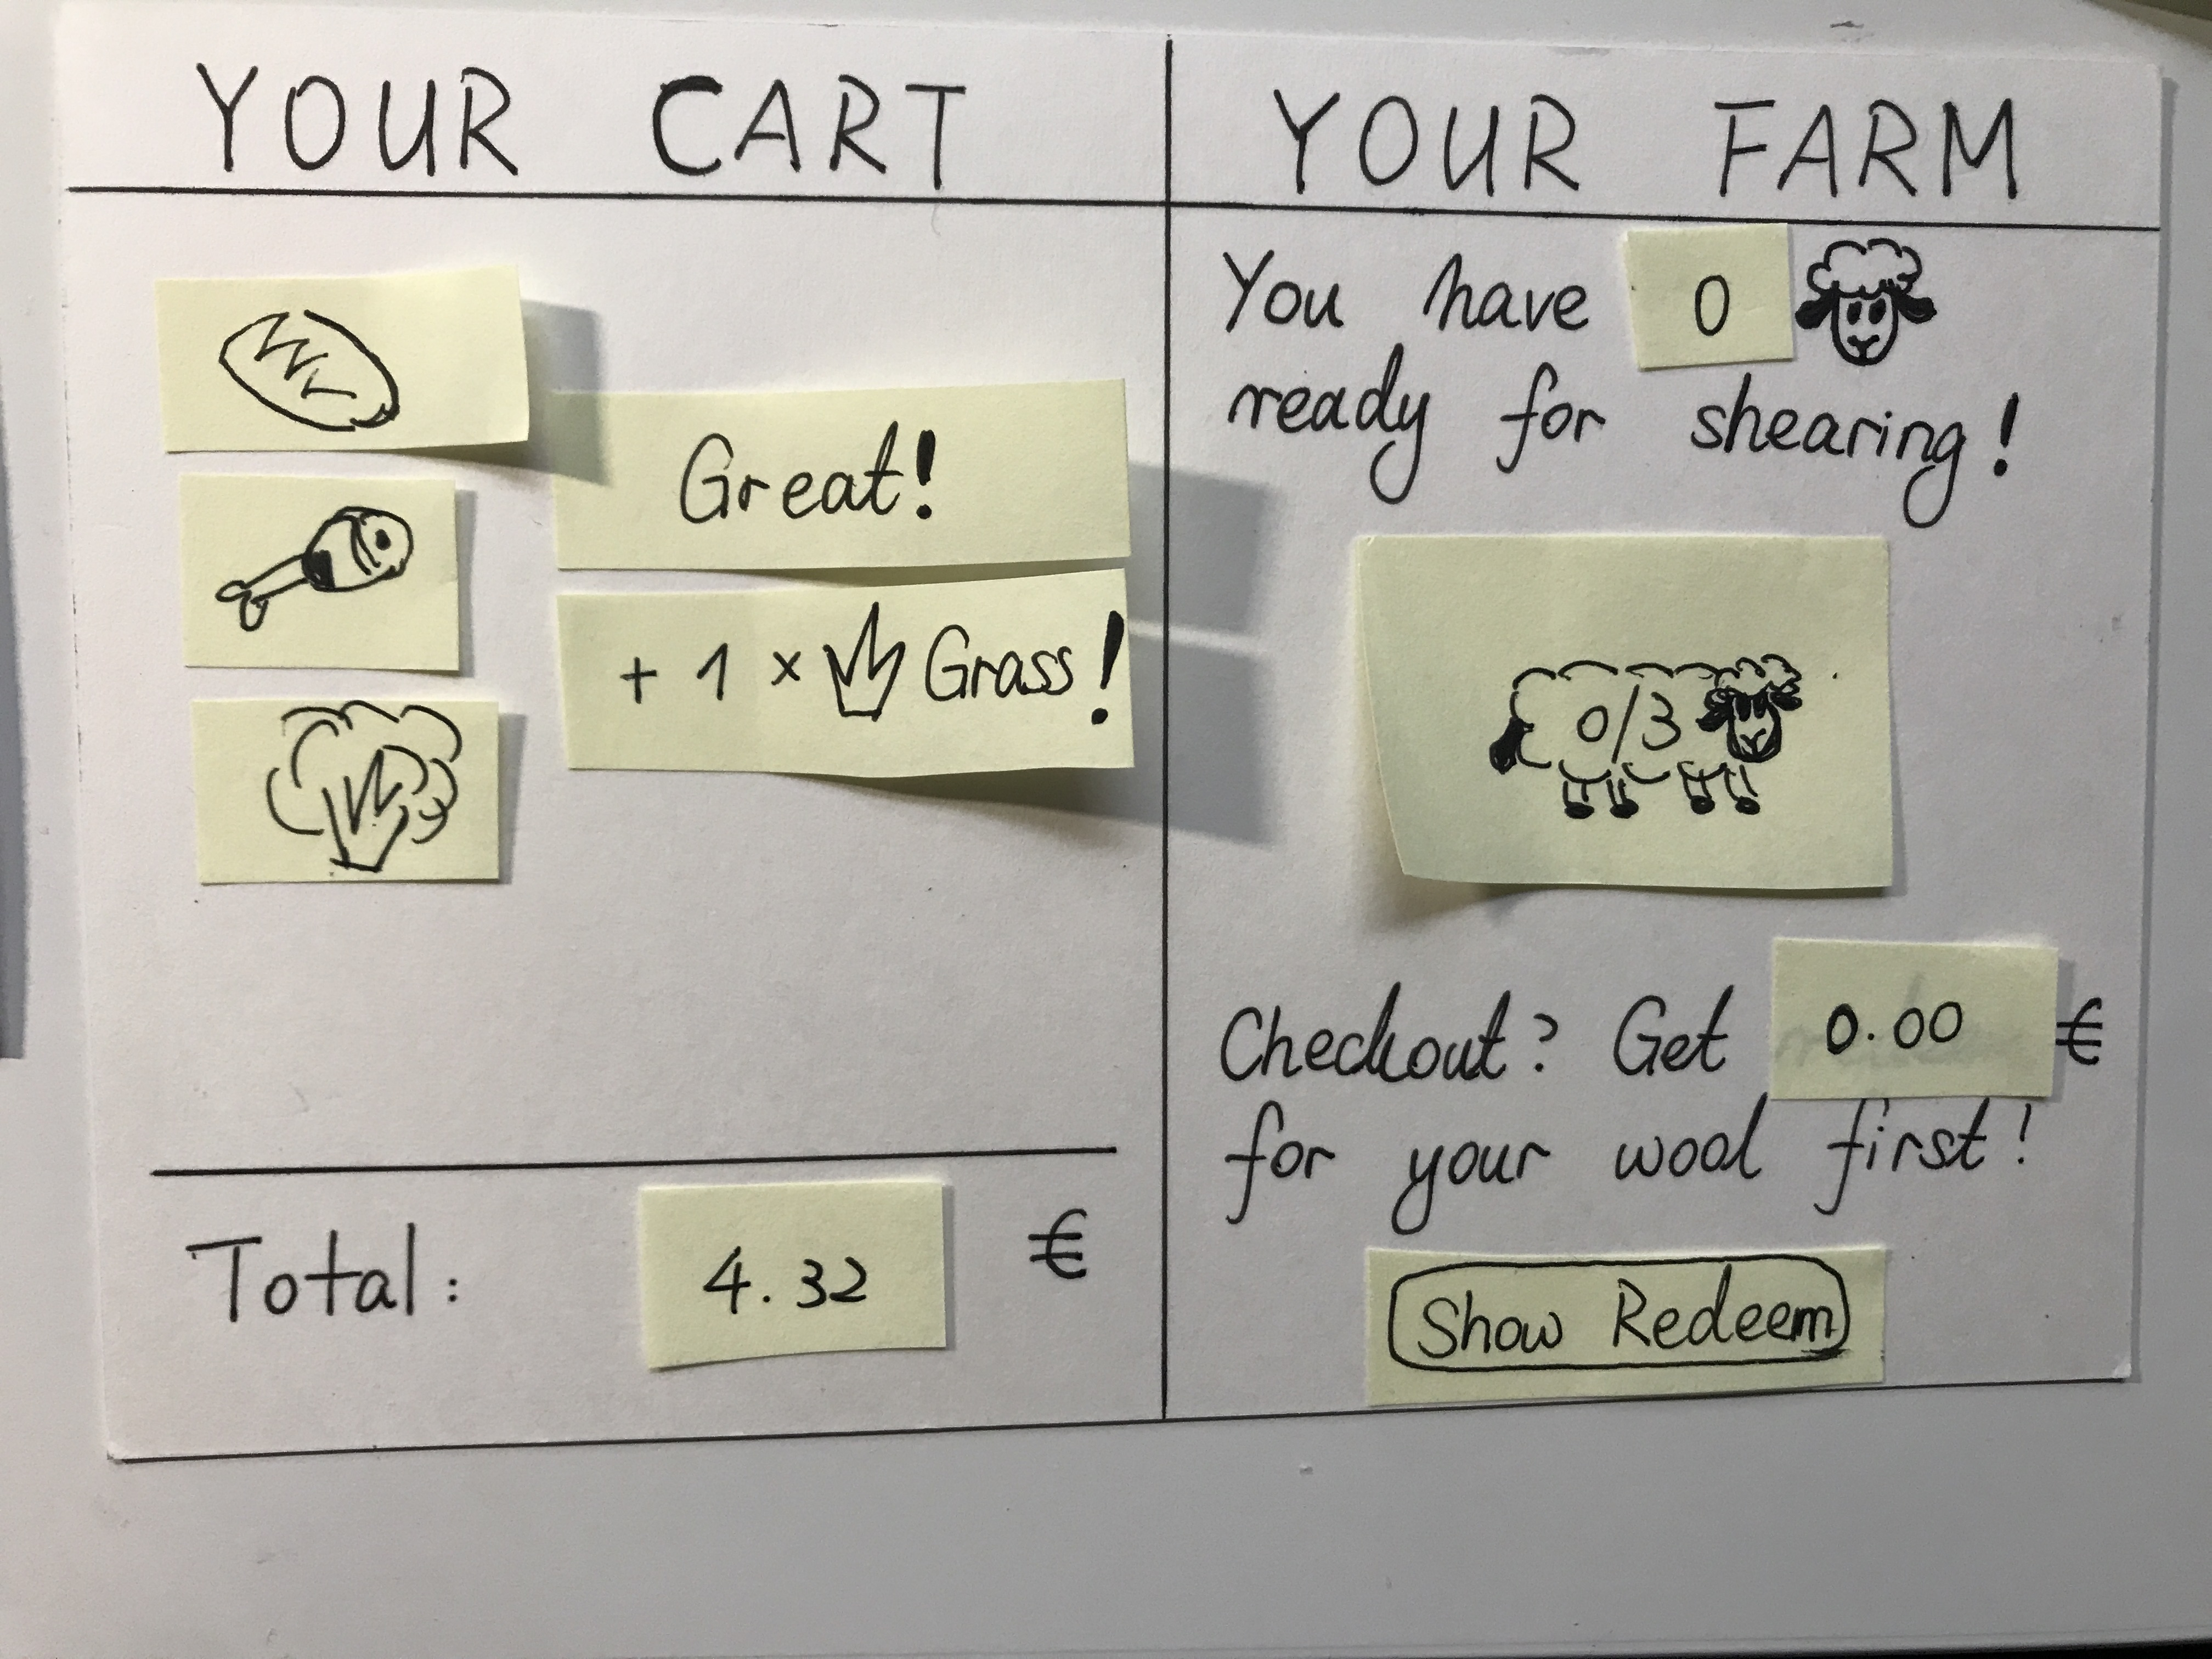
\includegraphics[scale=0.10, clip, trim={0em 0em 0em 0em}]{images/IMG_0572.jpg}
\end{figure}

\begin{figure}[h]
	\centering
	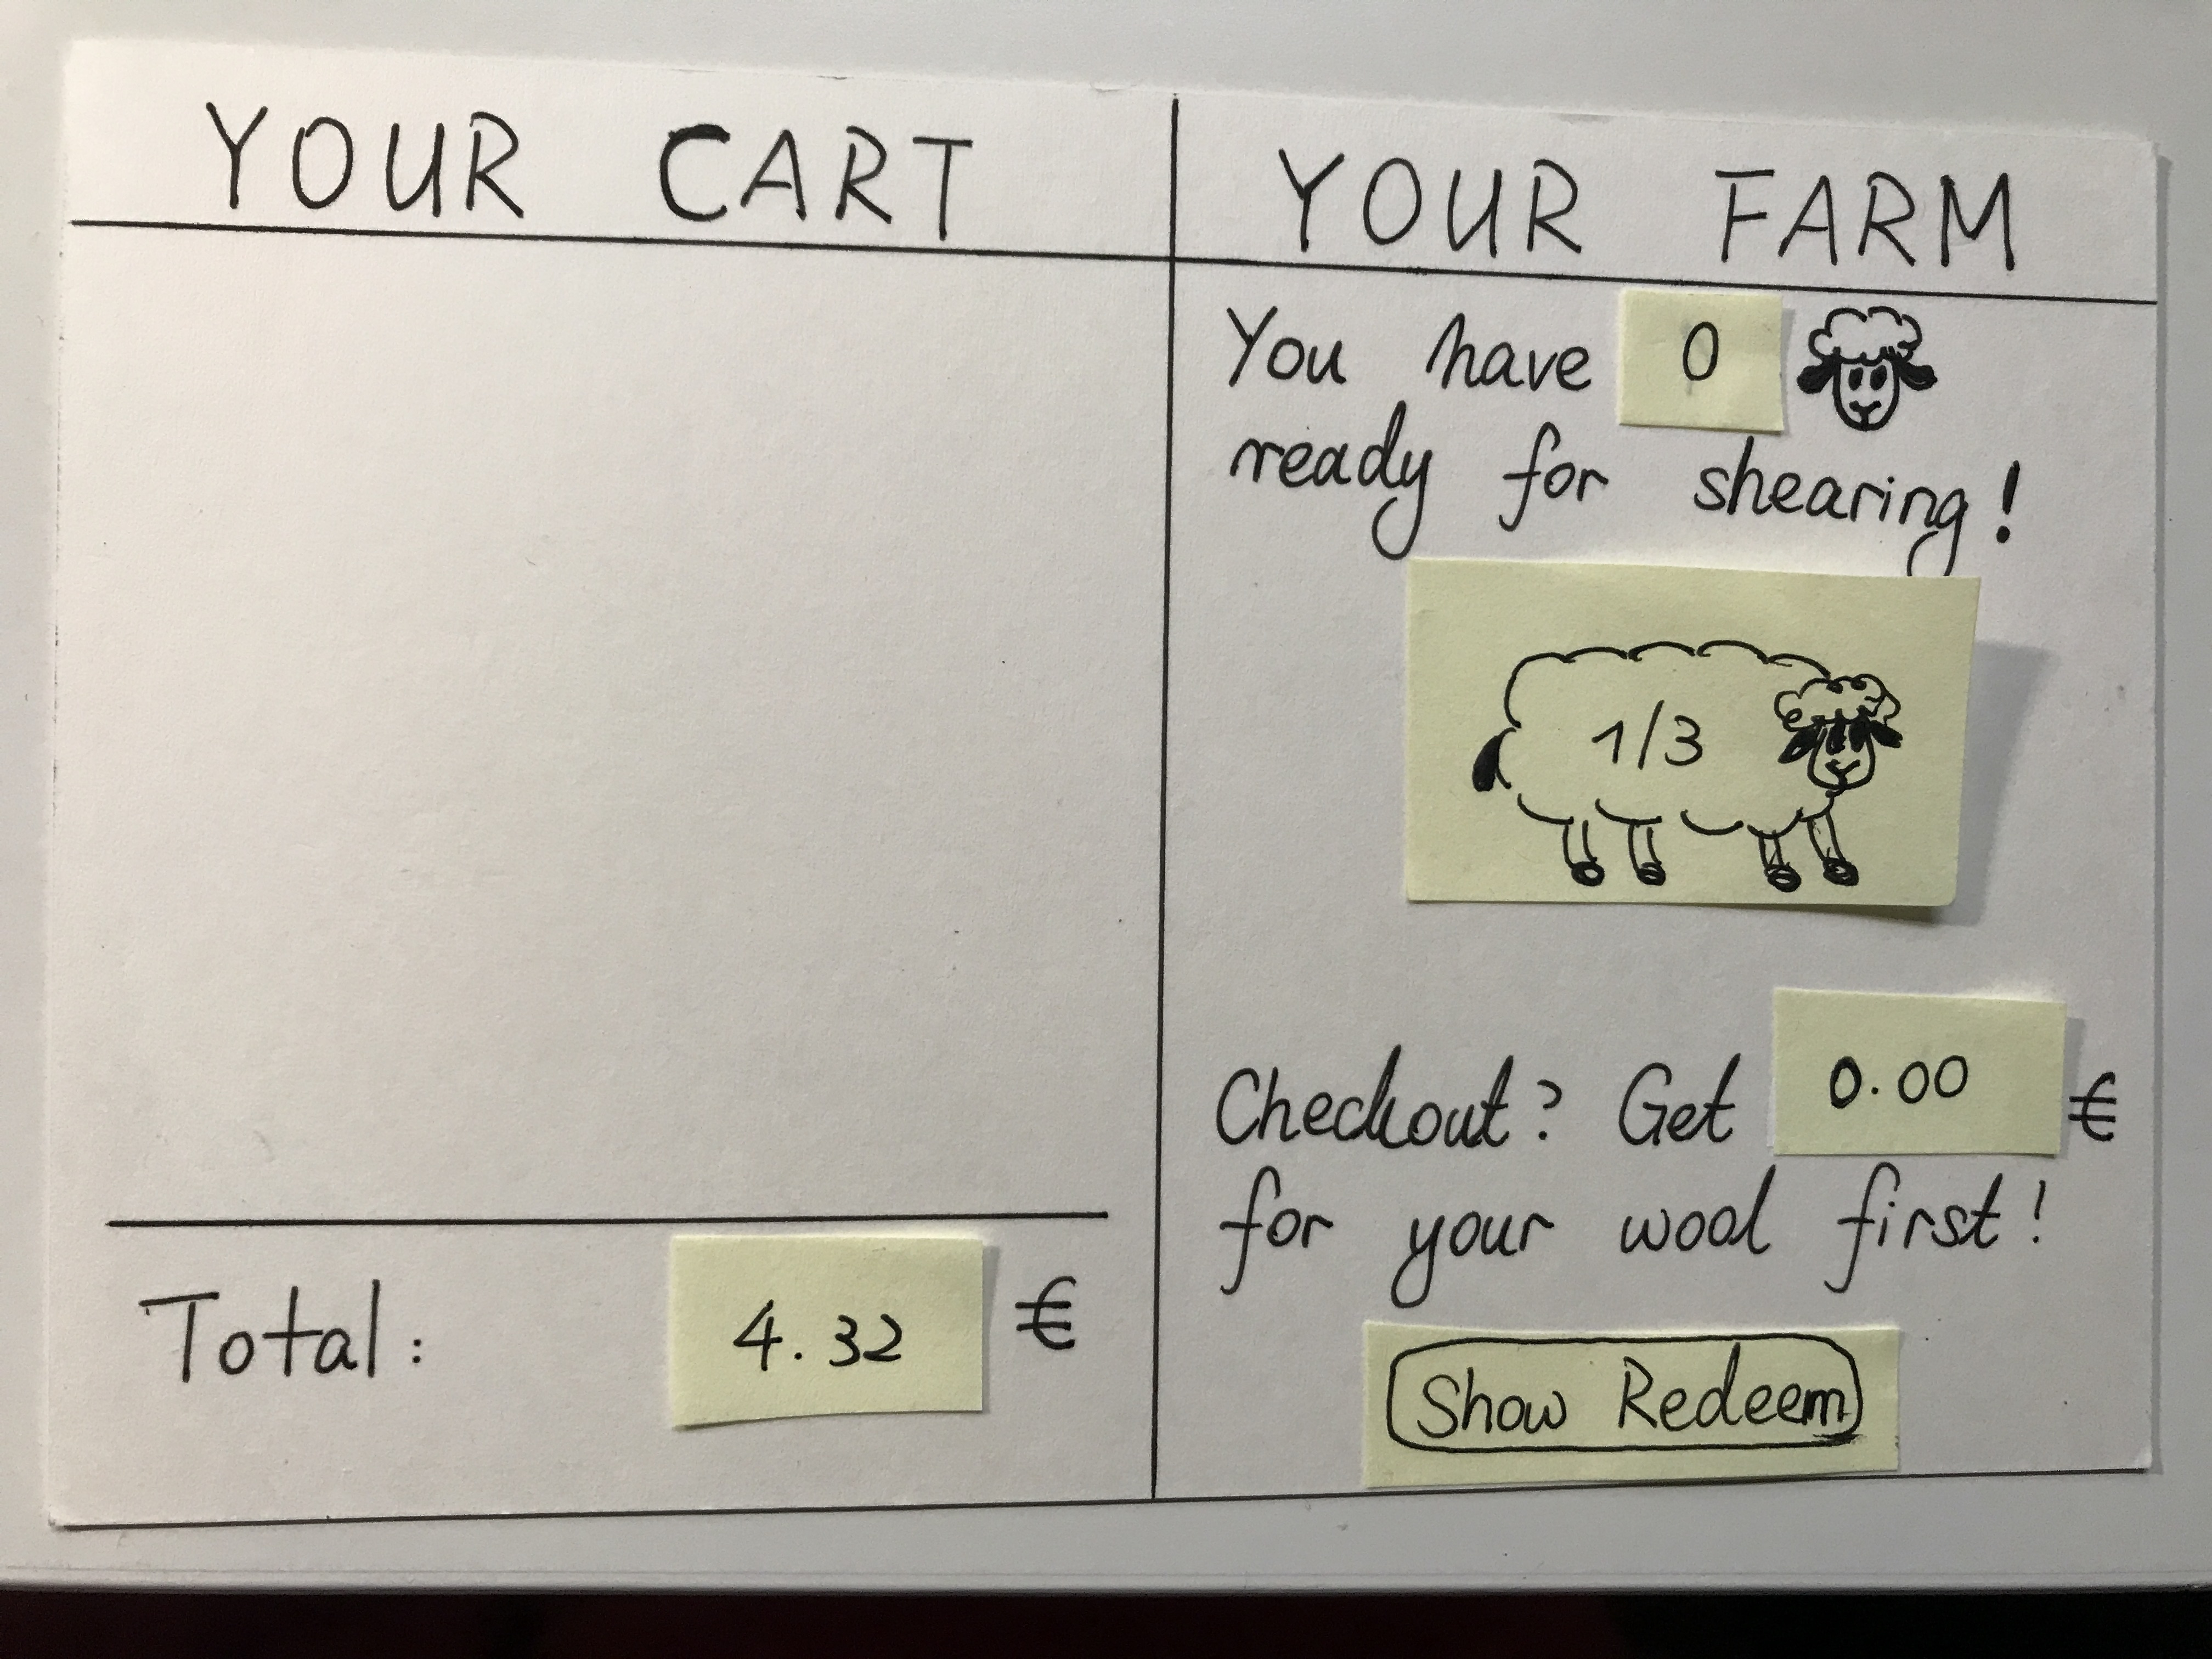
\includegraphics[scale=0.10, clip, trim={0em 0em 0em 0em}]{images/IMG_0576.jpg}
\end{figure}

\begin{figure}[h]
	\centering
	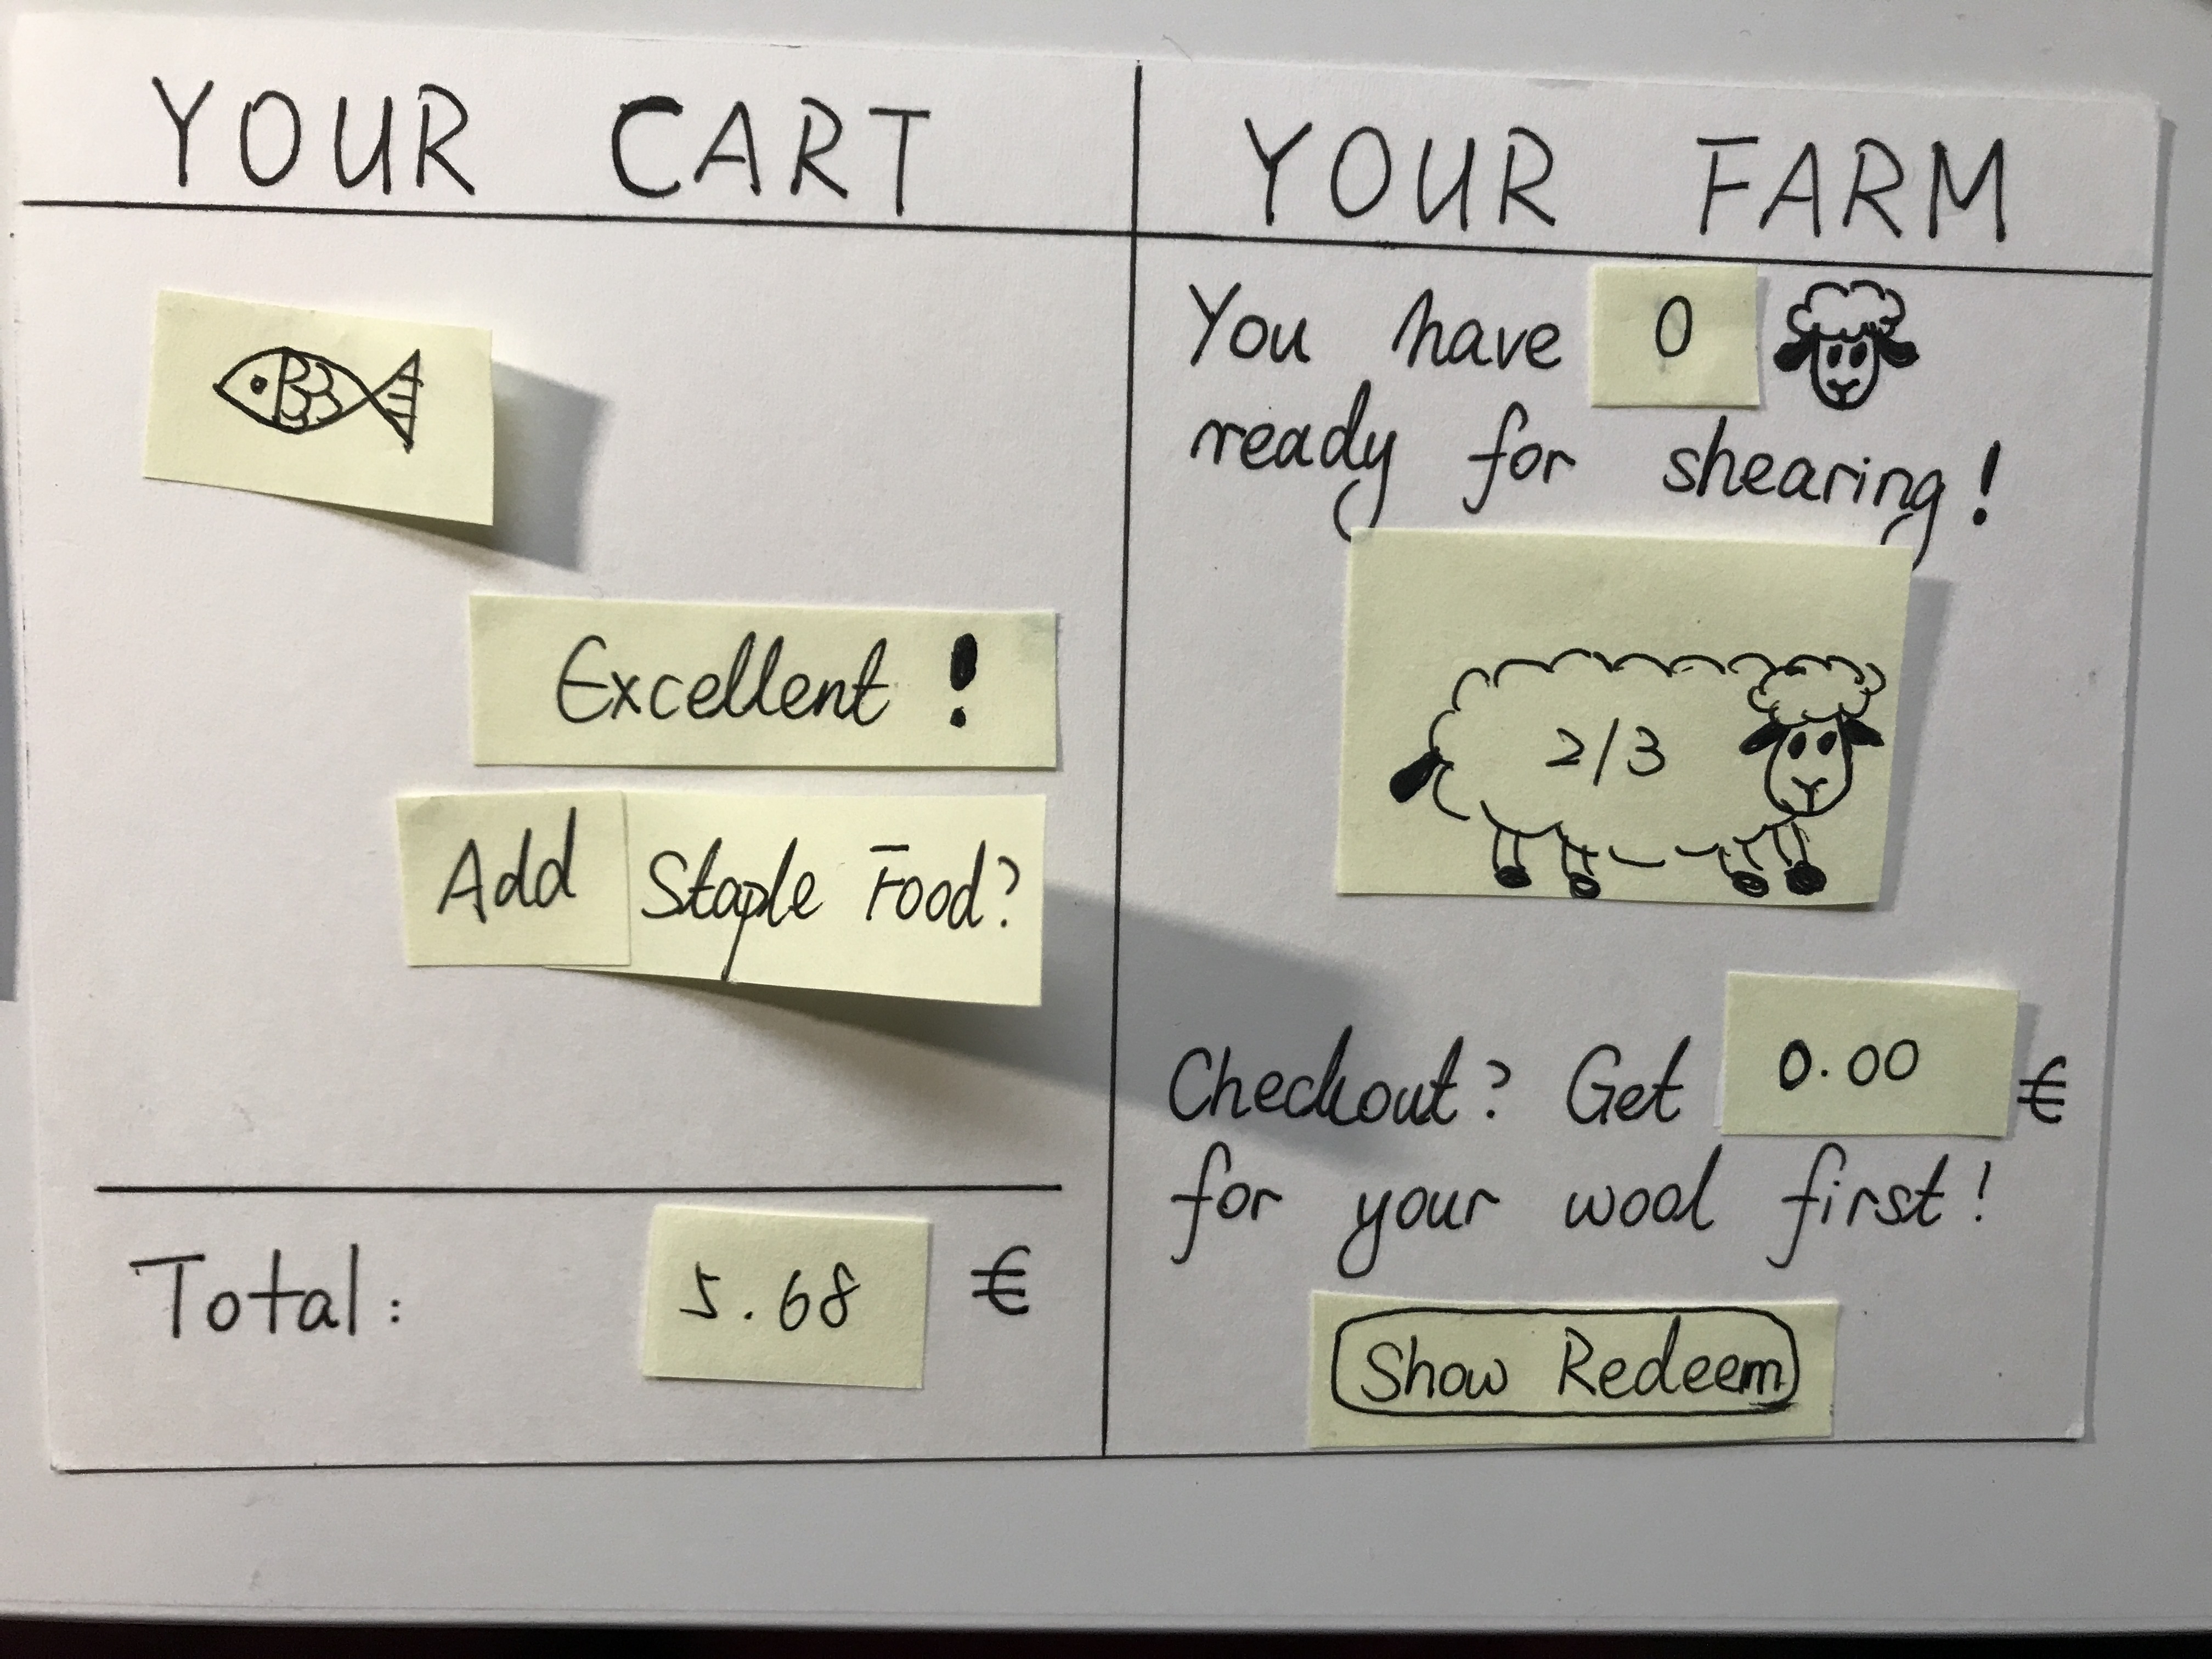
\includegraphics[scale=0.10, clip, trim={0em 0em 0em 0em}]{images/IMG_0577.jpg}
\end{figure}

\begin{figure}[h]
	\centering
	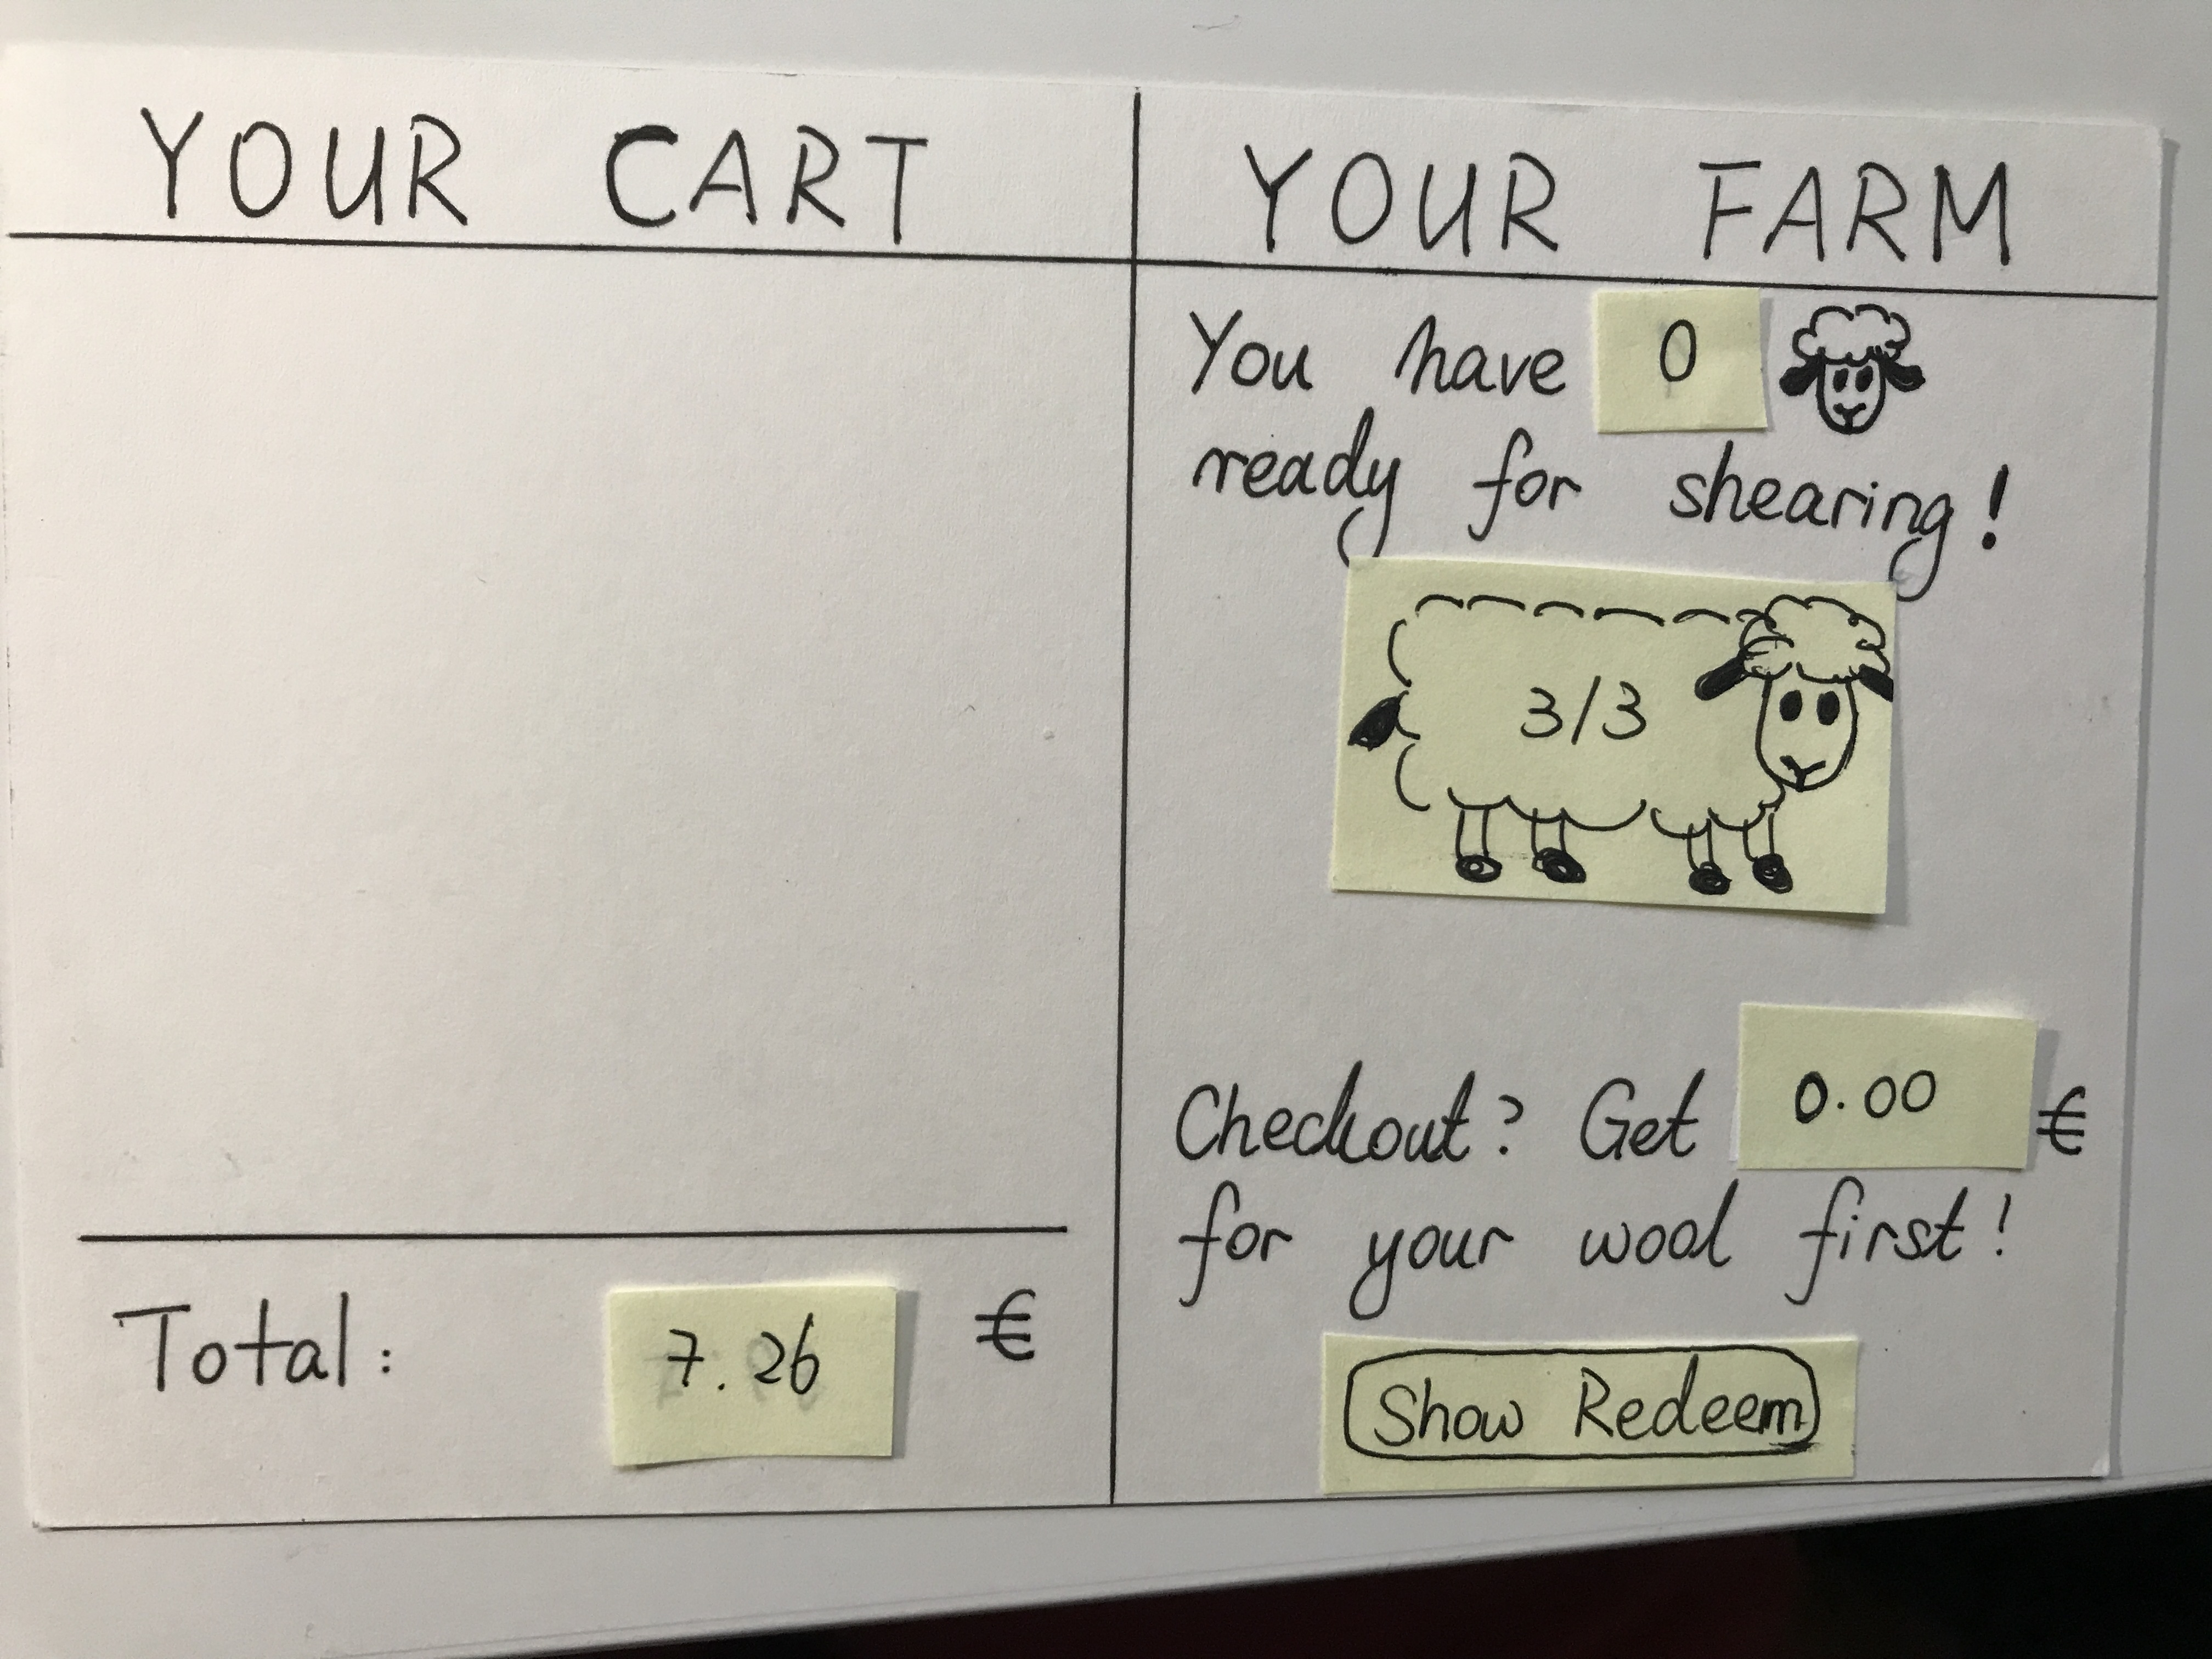
\includegraphics[scale=0.10, clip, trim={0em 0em 0em 0em}]{images/IMG_0578.jpg}
\end{figure}

\begin{figure}[h]
	\centering
	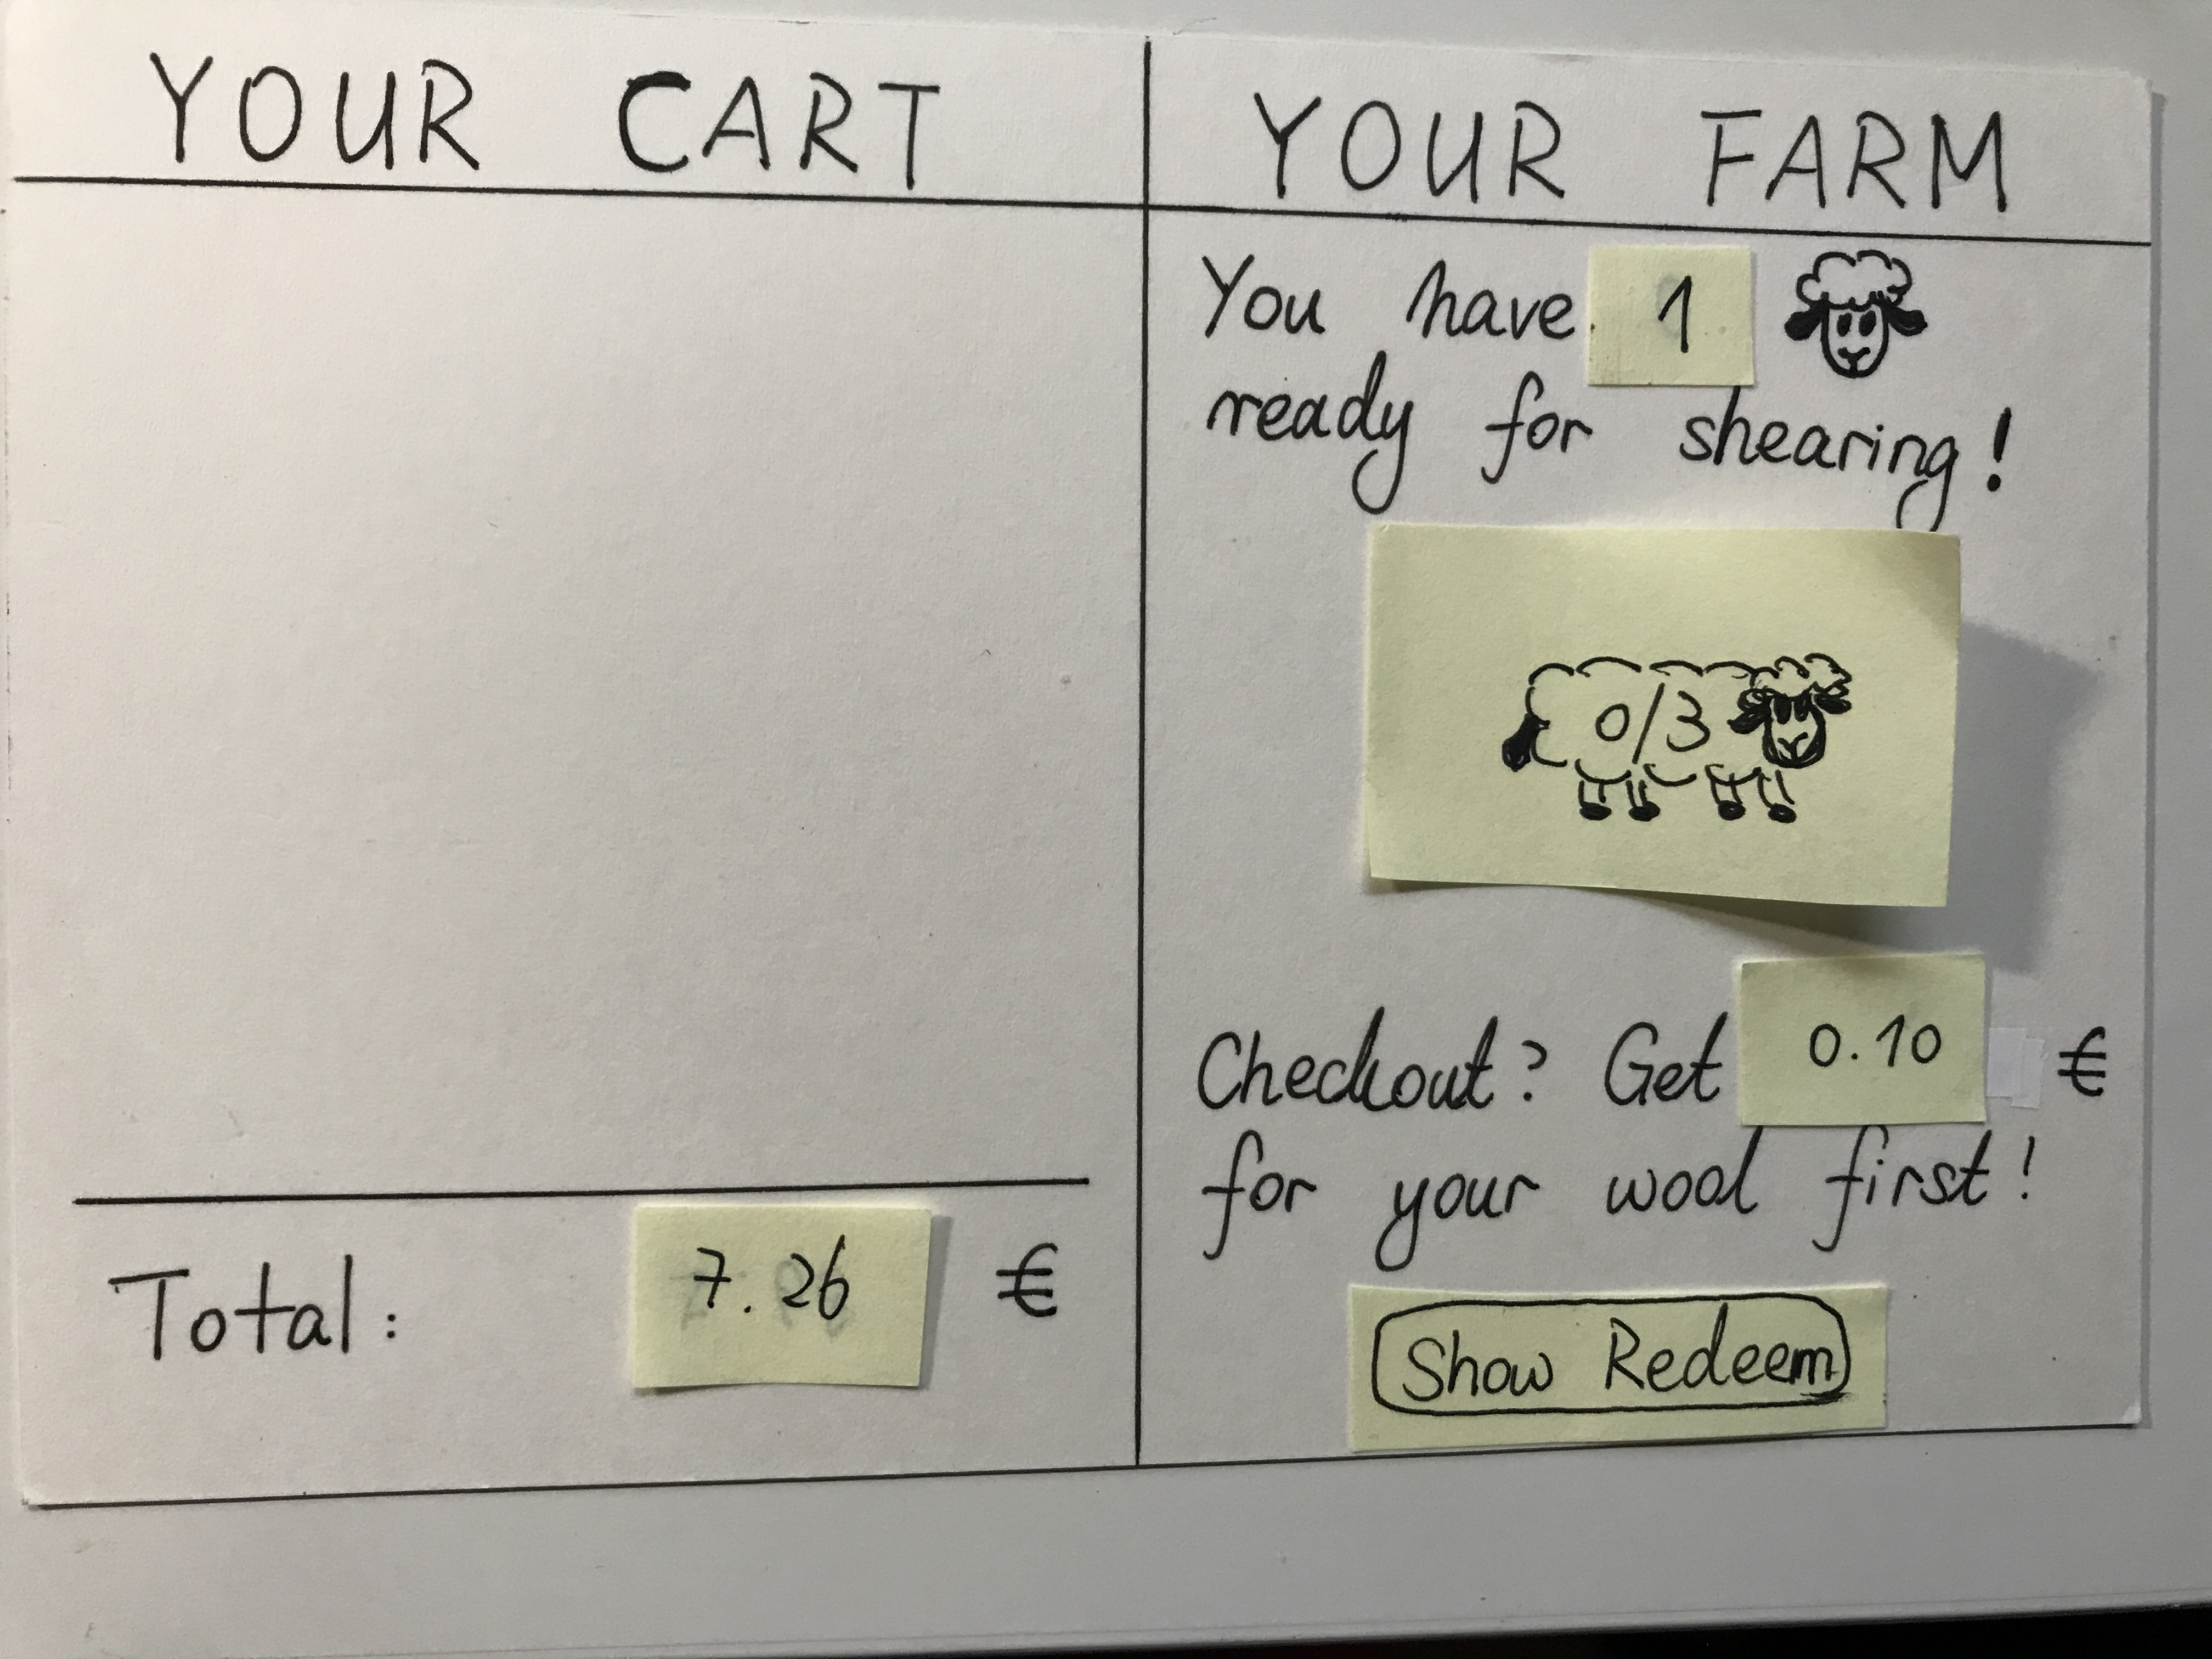
\includegraphics[scale=0.10, clip, trim={0em 0em 0em 0em}]{images/IMG_0579.jpg}
\end{figure}

\begin{figure}[h]
	\centering
	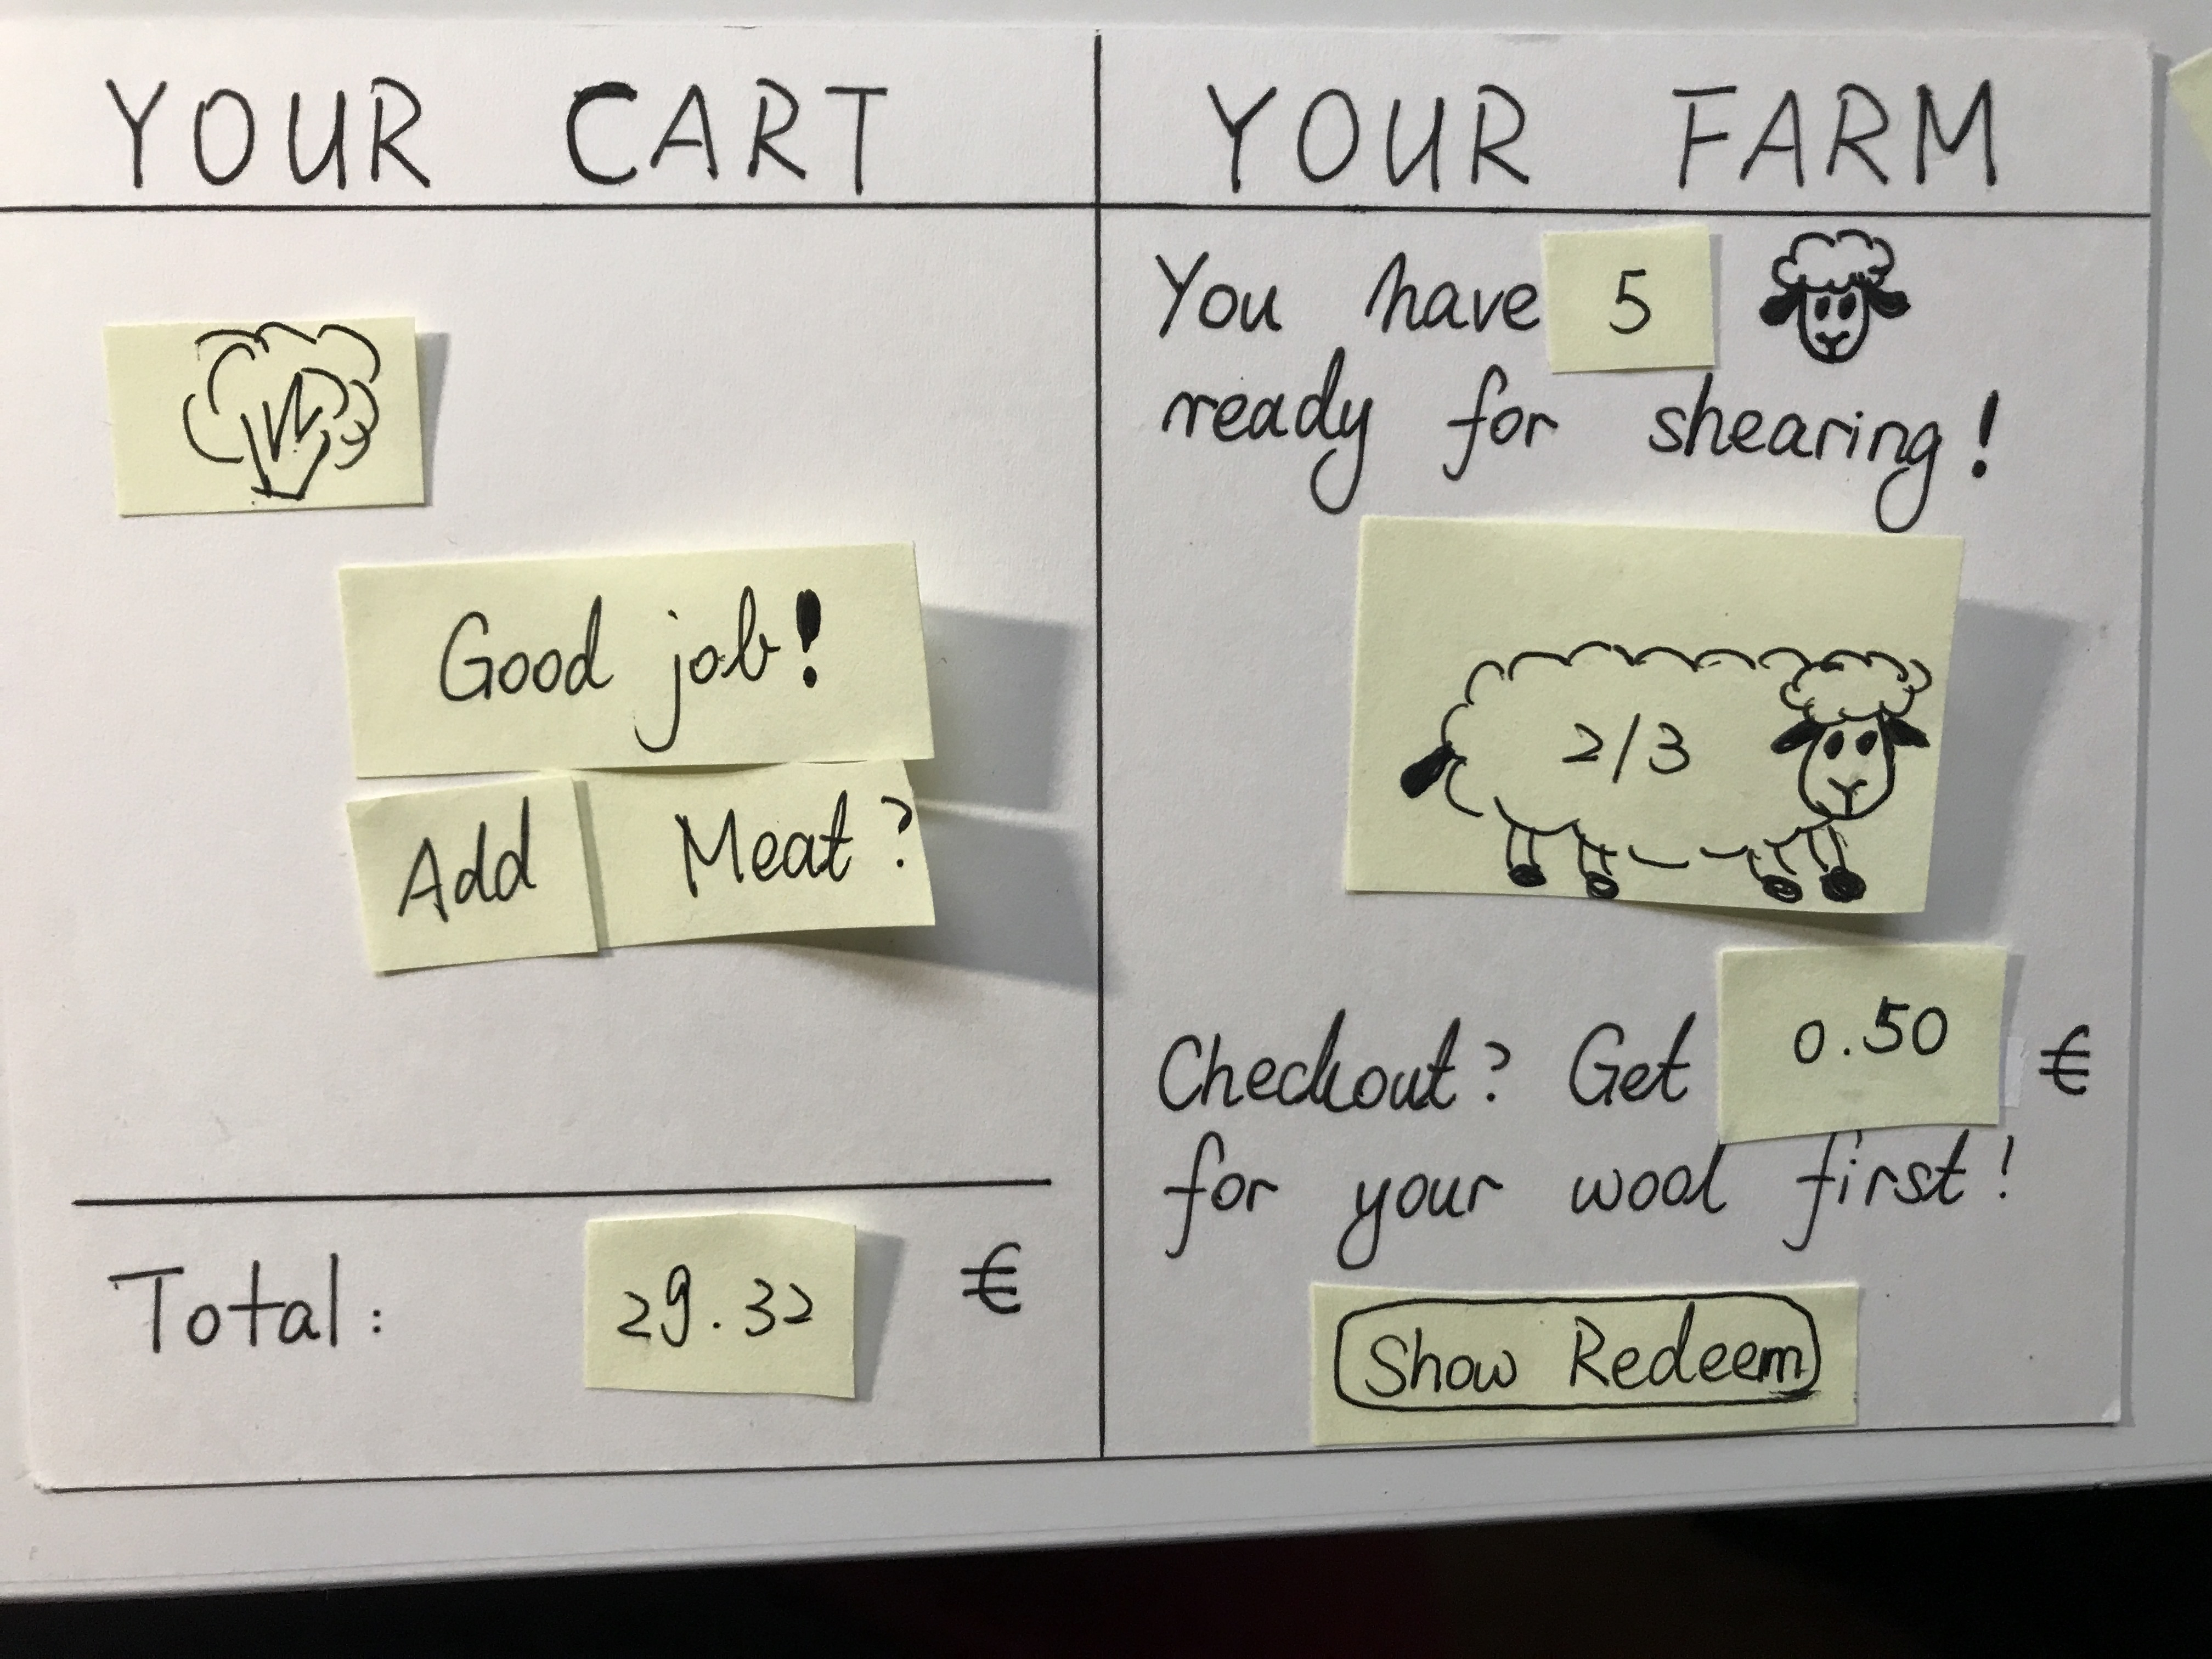
\includegraphics[scale=0.10, clip, trim={0em 0em 0em 0em}]{images/IMG_0580.jpg}
\end{figure}

\begin{figure}[h]
	\centering
	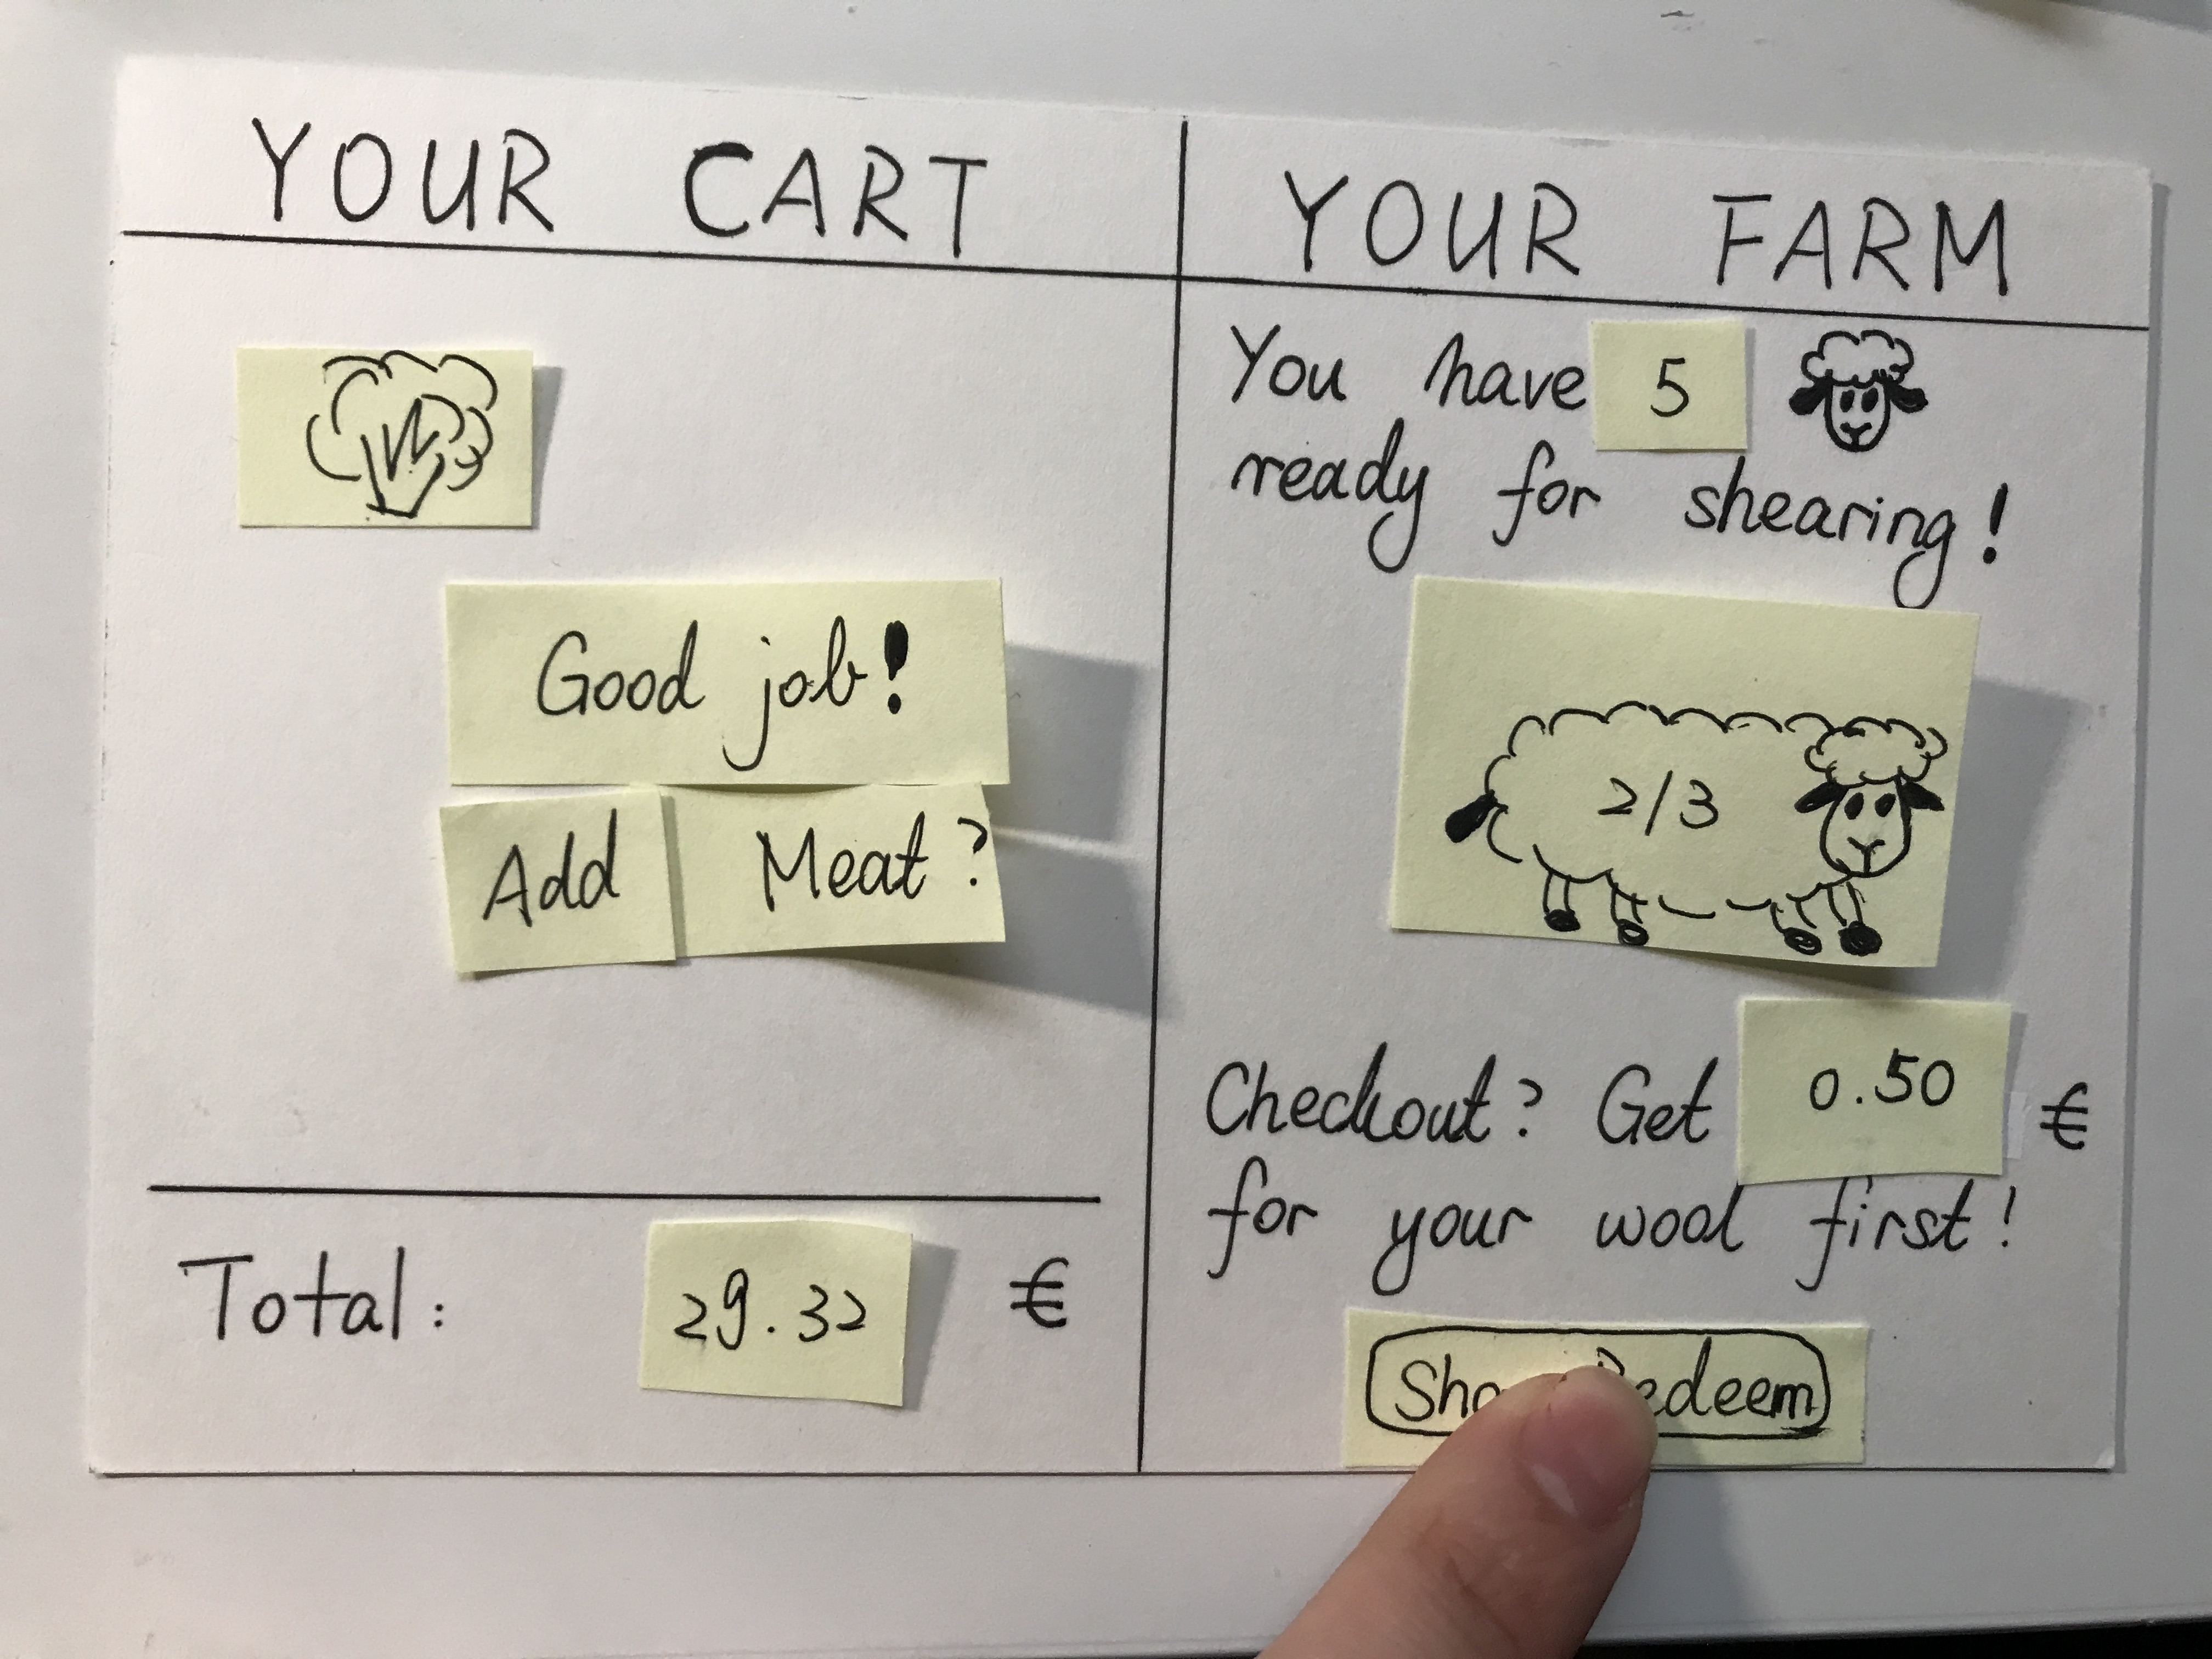
\includegraphics[scale=0.10, clip, trim={0em 0em 0em 0em}]{images/IMG_0581.jpg}
\end{figure}

\begin{figure}[h]
	\centering
	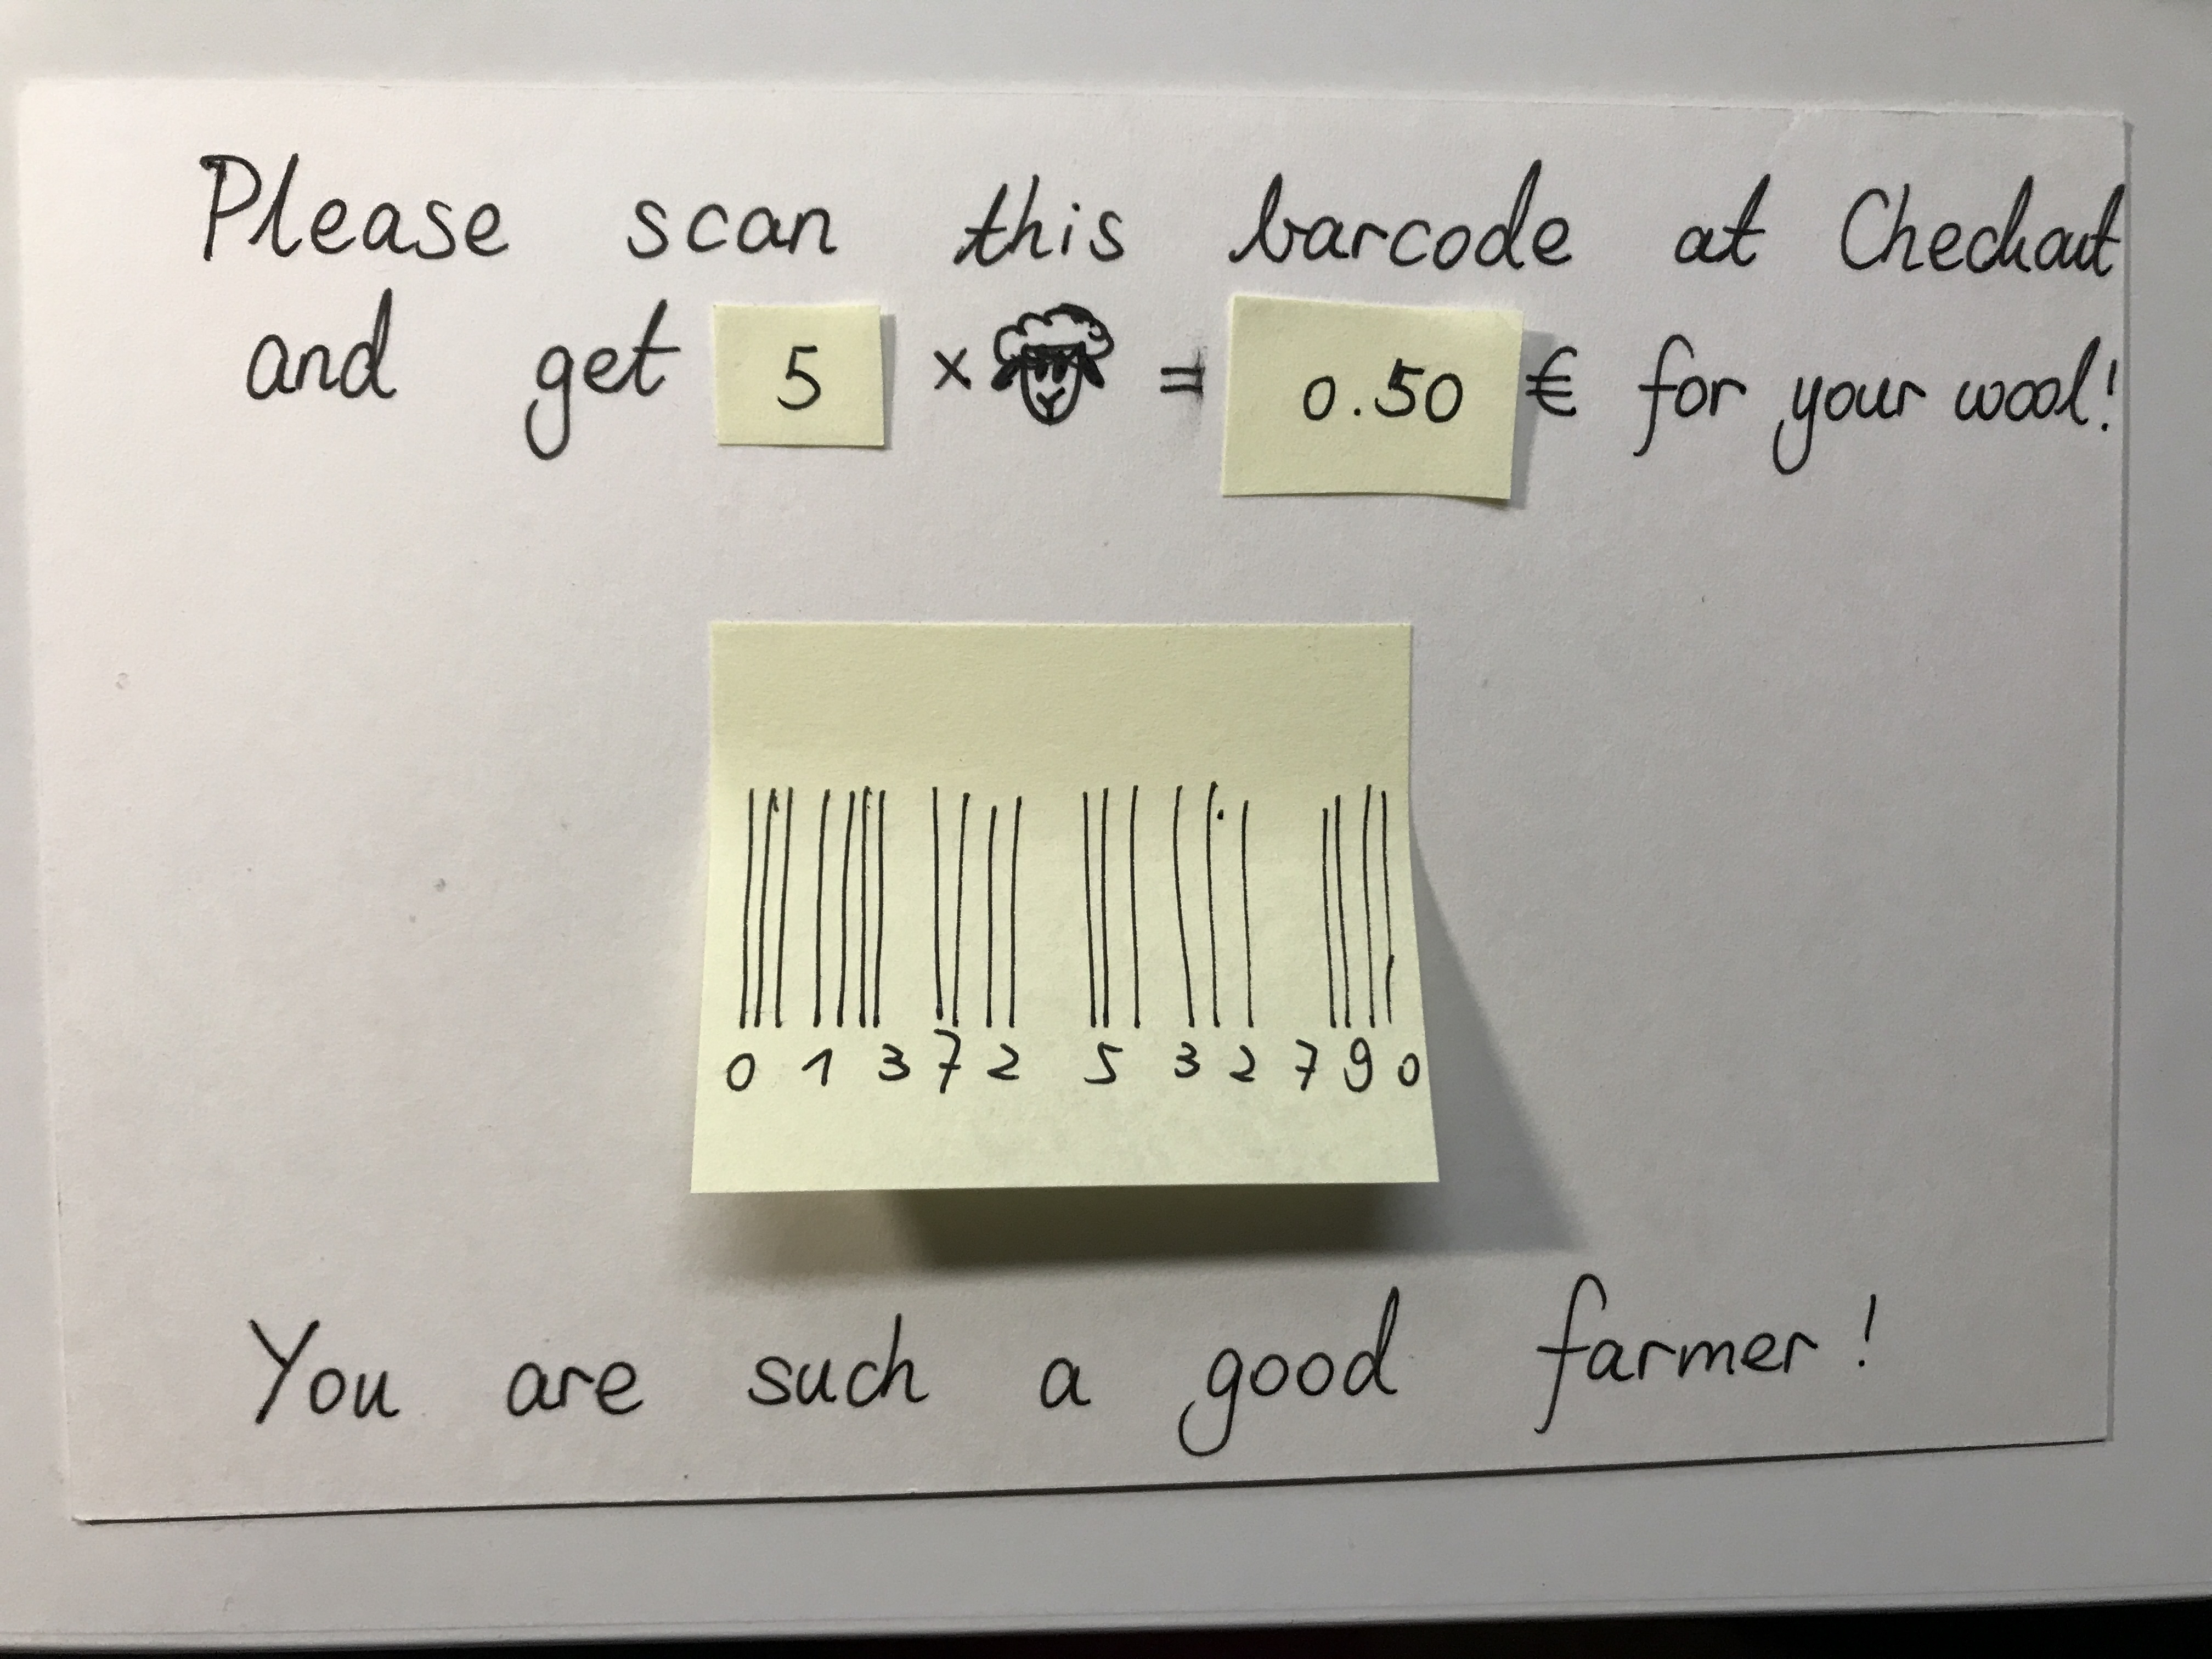
\includegraphics[scale=0.10, clip, trim={0em 0em 0em 0em}]{images/IMG_0582.jpg}
\end{figure}

\end{document}
